%===============================================================================
% LaTeX sjabloon voor de bachelorproef toegepaste informatica aan HOGENT
% Meer info op https://github.com/HoGentTIN/bachproef-latex-sjabloon
%===============================================================================

\documentclass{bachproef-tin}

\usepackage{hogent-thesis-titlepage} % Titelpagina conform aan HOGENT huisstijl

%%---------- Documenteigenschappen ---------------------------------------------
% TODO: Vul dit aan met je eigen info:

% De titel van het rapport/bachelorproef
\title{Een chatbot automatisch laten bijleren op basis van
	het gedrag van gebruikers}

% Je eigen naam
\author{Ivor Faingnaert}

% De naam van je promotor (lector van de opleiding)
\promotor{Leen Vuyge}

% De naam van je co-promotor. Als je promotor ook je opdrachtgever is en je
% dus ook inhoudelijk begeleidt (en enkel dan!), mag je dit leeg laten.
\copromotor{Sander Goossenss}

% Indien je bachelorproef in opdracht van/in samenwerking met een bedrijf of
% externe organisatie geschreven is, geef je hier de naam. Zoniet laat je dit
% zoals het is.
\instelling{Endare}

% Academiejaar
\academiejaar{2018-2019}

% Examenperiode
%  - 1e semester = 1e examenperiode => 1
%  - 2e semester = 2e examenperiode => 2
%  - tweede zit  = 3e examenperiode => 3
\examenperiode{2}

%===============================================================================
% Inhoud document
%===============================================================================

\begin{document}

%---------- Taalselectie -------------------------------------------------------
% Als je je bachelorproef in het Engels schrijft, haal dan onderstaande regel
% uit commentaar. Let op: de tekst op de voorkaft blijft in het Nederlands, en
% dat is ook de bedoeling!

%\selectlanguage{english}

%---------- Titelblad ----------------------------------------------------------
\inserttitlepage

%---------- Samenvatting, voorwoord --------------------------------------------
\usechapterimagefalse
%%=============================================================================
%% Voorwoord
%%=============================================================================

\chapter*{\IfLanguageName{dutch}{Woord vooraf}{Preface}}
\label{ch:voorwoord}

%% TODO:
%% Het voorwoord is het enige deel van de bachelorproef waar je vanuit je
%% eigen standpunt (``ik-vorm'') mag schrijven. Je kan hier bv. motiveren
%% waarom jij het onderwerp wil bespreken.
%% Vergeet ook niet te bedanken wie je geholpen/gesteund/... heeft

Het onderwerp van deze bachelorproef kwam ter sprake met nog een aantal andere onderwerpen die Endare, mijn stagebedrijf wou onderzoeken. Dit onderwerp gaande over chatbots sprak mij onmiddellijk aan door de enorme groei van AI en Machine learning. Ook chatbots is een onderdeel hiervan dus leek het mij interessant om hier dieper op in te gaan en dit te onderzoeken. Chatbots zullen meer en meer worden gebruikt in de toekomst. De ontwikkeling van chatbots met AI staan nog niet zo super ver en daardoor wou ik mij daar ook wat meer in verdiepen en een meerwaarde bieden in dit domein.

Ik zou graag de personen willen bedankten die mij hebben geholpen bij het realiseren van deze bachelorproef. Mijn promotor Leen Vuyge voor mij zo goed te gegeleiden tijdens dit onderzoek en altijd tijd vrij te maken om samen te zitten en mij zo goed mogelijk al mijn vragen uit te leggen.

Ook zou ik mijn co-promoter Sander Goossens willen bedanken voor de hulp en de verduidelijking van dit onderzoek. Hij heeft mij geholpen met het zoeken van een onderwerp, het verduidelijken van vragen en problemen die ik had en de tijd voor samen te denken voor een oplossing op de onderzoeksvraag.

Als laatste zou ik mijn ouders en grootvader willen bedanken voor het nalezen en controleren van deze bachelorproef. Ook voor de grote steun tijdens het schrijven van deze.

%%=============================================================================
%% Samenvatting
%%=============================================================================

% TODO: De "abstract" of samenvatting is een kernachtige (~ 1 blz. voor een
% thesis) synthese van het document.
%
% Deze aspecten moeten zeker aan bod komen:
% - Context: waarom is dit werk belangrijk?
% - Nood: waarom moest dit onderzocht worden?
% - Taak: wat heb je precies gedaan?
% - Object: wat staat in dit document geschreven?
% - Resultaat: wat was het resultaat?
% - Conclusie: wat is/zijn de belangrijkste conclusie(s)?
% - Perspectief: blijven er nog vragen open die in de toekomst nog kunnen
%    onderzocht worden? Wat is een mogelijk vervolg voor jouw onderzoek?
%
% LET OP! Een samenvatting is GEEN voorwoord!

%%---------- Nederlandse samenvatting -----------------------------------------
%
% TODO: Als je je bachelorproef in het Engels schrijft, moet je eerst een
% Nederlandse samenvatting invoegen. Haal daarvoor onderstaande code uit
% commentaar.
% Wie zijn bachelorproef in het Nederlands schrijft, kan dit negeren, de inhoud
% wordt niet in het document ingevoegd.

\IfLanguageName{english}{%
\selectlanguage{dutch}
\chapter*{Samenvatting}
\lipsum[1-4]
\selectlanguage{english}
}{}

%%---------- Samenvatting -----------------------------------------------------
% De samenvatting in de hoofdtaal van het document

\chapter*{\IfLanguageName{dutch}{Samenvatting}{Abstract}}

Dit werk is belangrijk voor het makkelijker maken van de ontwikkeling van een chatbot. Grotendeels zal dit onderzocht worden voor het besparen van tijd en het beter maken van de accuraatheid van deze bot.

Omdat het ontwikkelen van een chatbot zeer veel tijd in beslag neemt, vooral het op punt stellen van de accuraatheid van de bot. Er zal dus een efficiëntere manier gezocht worden om deze bot dingen aan te leren.

Er is een proof of concept werkende met LUIS opgesteld die de inputs van de gebruiker opvangt, deze controleerd aan de hand van de info die LUIS voorziet per input. Als de input na deze controle is goedgekeurd zal deze input automatisch worden gelinkt aan de juiste intent en zal de manuele controle achterwege kunnen worden gelaten.

In dit document bevindt zich een onderzoek van een aantal van de bekendste NLP-frameworks. Er wordt onderzocht hoe deze precies werken en of de API toegankelijk genoeg is voor het realiseren van deze proof of concept.

Het resultaat van dit onderzoek is positief uitgevallen. Het is effectief gelukt met LUIS om een proof of concept op te stellen die via de API LUIS gedeeltelijk automatisch zal aanleren.

Uit de testen hiervan is gebleken dat maar liefst 50 percent van de inputs niet meer in de 'Review endpoint utterances' tabblad komen maar automarisch worden gelinkt aan de correcte intent.

In een vervolgonderzoek kan dit onderzoek nog wat uitgebreid worden. Er kunnen met meerdere LUIS-apps gewerkt worden, met elk een totaal onder doel en onderwerp. Deze kunnen getest worden met meerdere en verschillende testdata. Ook kan er een veel ingewikkeldere applicatie getest worden met moeilijkere intent die utterances hebben met veel meer entities en controleren of deze hier ook correct worden gelinkt.

%---------- Inhoudstafel -------------------------------------------------------
\pagestyle{empty} % Geen hoofding
\tableofcontents  % Voeg de inhoudstafel toe
\cleardoublepage  % Zorg dat volgende hoofstuk op een oneven pagina begint
\pagestyle{fancy} % Zet hoofding opnieuw aan

%---------- Lijst figuren, afkortingen, ... ------------------------------------

% Indien gewenst kan je hier een lijst van figuren/tabellen opgeven. Geef in
% dat geval je figuren/tabellen altijd een korte beschrijving:
%
%  \caption[korte beschrijving]{uitgebreide beschrijving}
%
% De korte beschrijving wordt gebruikt voor deze lijst, de uitgebreide staat bij
% de figuur of tabel zelf.

\listoffigures
\listoftables

% Als je een lijst van afkortingen of termen wil toevoegen, dan hoort die
% hier thuis. Gebruik bijvoorbeeld de ``glossaries'' package.
% https://www.overleaf.com/learn/latex/Glossaries

%---------- Kern ---------------------------------------------------------------

% De eerste hoofdstukken van een bachelorproef zijn meestal een inleiding op
% het onderwerp, literatuurstudie en verantwoording methodologie.
% Aarzel niet om een meer beschrijvende titel aan deze hoofstukken te geven of
% om bijvoorbeeld de inleiding en/of stand van zaken over meerdere hoofdstukken
% te verspreiden!

%%=============================================================================
%% Inleiding
%%=============================================================================

\chapter{\IfLanguageName{dutch}{Inleiding}{Introduction}}
\label{ch:inleiding}

In dit onderdeel zal er al een beter beeld worden geschept over het onderwerp zelf en of dit de moeite waard is om te onderzoeken.

\section{\IfLanguageName{dutch}{Probleemstelling}{Problem Statement}}
\label{sec:probleemstelling}

Wanneer een bedrijf zoals Endare, de opdrachtgever van deze onderzoeksvraag een chatbot ontwikkelt voor een klant, zal er veel werk nodig zijn in het op punt zetten van deze chatbot. Een deel van dit werk zal pas kunnen worden gedaan wanneer de chatbot effectief in gebruik is genomen. Al de input dat gebruikers ingeven waarvan LUIS zelf maar een beetje aan twijfelt zal moeten manueel gelinkt worden aan de juiste intent. Door een antwoord te zoeken op de onderzoeksvraag zal dit werk worden verminderd door een gedeelte van deze inputs automatisch te koppelen aan de juiste intent.

\section{\IfLanguageName{dutch}{Onderzoeksvraag}{Research question}}
\label{sec:onderzoeksvraag}

De onderzoeksvraag 'Kunnen we een chatbot automatisch laten bijleren op basis van het gedrag van gebruikers?', zal in deze bachelorproef onderzocht worden. Kan hier door middel van de input die gebruikers ingeven via de chatbot, deze input automatisch worden gelinkt aan de correcte intent, dus de bot laten bijleren. Hierbij zal ook onderzocht worden in welke mate dit automatisch zal gebeuren en het werk voor het ontwikkelteam verminderen.

\section{\IfLanguageName{dutch}{Onderzoeksdoelstelling}{Research objective}}
\label{sec:onderzoeksdoelstelling}

Dit werk zal een succes zijn als de API van minstens één van de onderzochte frameworks toelaat dat een input van een gebruiker kan opgehaald en gecontroleerd worden om dit dan te linken aan de correcte intent. Er zal een proof of concept worden opgesteld om dit te realiseren.

\section{\IfLanguageName{dutch}{Opzet van deze bachelorproef}{Structure of this bachelor thesis}}
\label{sec:opzet-bachelorproef}

% Het is gebruikelijk aan het einde van de inleiding een overzicht te
% geven van de opbouw van de rest van de tekst. Deze sectie bevat al een aanzet
% die je kan aanvullen/aanpassen in functie van je eigen tekst.

De rest van deze bachelorproef is als volgt opgebouwd:

In Hoofdstuk~\ref{ch:stand-van-zaken} wordt een overzicht gegeven van de stand van zaken binnen het onderzoeksdomein, op basis van een literatuurstudie.

In Hoofdstuk~\ref{ch:methodologie} wordt de methodologie toegelicht en worden de gebruikte onderzoekstechnieken besproken om een antwoord te kunnen formuleren op de onderzoeksvragen.

% TODO: Vul hier aan voor je eigen hoofstukken, één of twee zinnen per hoofdstuk

In Hoofdstuk~\ref{ch:poc} wordt de gemaakte proof of concept besproken. Hierin wordt ook gezien hoe het gekozen framework zal worden opgezet.

In Hoofdstuk~\ref{ch:res} zal de accuraatheid en de efficiëntie van de proof of concept worden getest.

In Hoofdstuk~\ref{ch:conclusie} tenslotte, wordt de conclusie gegeven en een antwoord geformuleerd op de onderzoeksvragen. Daarbij wordt ook een aanzet gegeven voor toekomstig onderzoek binnen dit domein.
\chapter{\IfLanguageName{dutch}{Stand van zaken}{State of the art}}
\label{ch:stand-van-zaken}

% Tip: Begin elk hoofdstuk met een paragraaf inleiding die beschrijft hoe
% dit hoofdstuk past binnen het geheel van de bachelorproef. Geef in het
% bijzonder aan wat de link is met het vorige en volgende hoofdstuk.

% Pas na deze inleidende paragraaf komt de eerste sectiehoofding.

In dit onderdeel zal de werking worden uitgelegd van een chatbot. Er zullen ook enkele van de meest bekende frameworks vergeleken worden met mekaar.

\section{Chatbot}
\label{sec:Chatbot}

Een chatbot is software die gemaakt is voor het automatiseren van een bepaalde taak. Er kan met de chatbot geconverseerd worden via een gebruikers interface. Deze chatbot heeft op zich toegang tot bepaalde data die toegankelijk is via een API zodat het deze kan leveren aan een bepaalde gebruiker die hier om vraagt.

De gebruikers interfaces kunnen zich bevinden op Messenger, Skype, Slack, WhatsApp, enz. Ook Siri en Alexa zijn bots, ze variëren van een chatfunctie tot een spraakassistent. Het is de bedoeling dat de gebruiker een vraag intypt en de chatbot geeft daar zo een gepast mogelijk antwoord op. Een chatbot kan zelf ook altijd een vraag stellen, dat kan zijn voor de naam van de persoon te weten te komen, zodat deze bot persoonlijker kan antwoorden. Het kan ook zijn voor een quiz of iets dergelijks.

Met NLP en machine learning is het mogelijk om mensentaal aan een chatbot aan te leren. Deze hebben een zeer grote rol bij het maken van zo een bot. ~\autocite{assaf2017}

\section{Soorten Chatbots}
\label{sec:Soorten Chatbots}

Chatbots kunnen onderverdeeld worden in verschillende categorieën.

\subsection{Rule-Bases Bots}
\label{Rule-Bases Bots}

Een rule based bot is een geautomatiseerde bot die reageert op bepaalde acties en sleutelwoorden en worden vaak ingezet op gespecialiseerde taken. Eén van de talen van zo een bot is AIML (Artificial Intelligence Markup Language), dat is een taal gebaseerd op XML. Deze laat toe om ontwikkelaars regels op te stellen voor een bot die deze moet volgen. Het is onmogelijk om regels te schrijven voor elk mogelijk scenario. ~\autocite{Kumar2017}

\subsection{AI-bot}
\label{AI-bot}

Een AI-bot simuleert het gedrag van een mens. Deze bot zal de bekende Turing-test moeten doorstaan. Deze test is ontwikkeld door Alan Turing in 1950. Hierin wordt gekeken of een mens onderscheid kan maken tussen een echte mens en een computer.

Deze bots zijn getraind aan de hand van een bepaalde hoeveelheid vragen. Voor elke vraag vindt de bot het meest relevante antwoord van alle mogelijke antwoorden. Zulke bots moeten ook rekening houden met de spelling en zinsbouw. Eenmaal deze ook goed getraind zijn daarop, zijn ze veel beter dan een rule-based bot.

\subsection{Generalistische bot}
\label{Generalistische bot}

Deze bots gebruiken vooral data uit databases en zoekmachines maar kunnen de gebruiker ook koppelen aan diensten. Deze heeft geen specifieke taak maar kan op een grote selectie van vragen antwoorden. Eénmaal de gebruiker iets specifieker in detail wil gaan over een bepaald onderwerp, kan deze bot overgaan naar een specialisatiebot.

\subsection{Specialisatiebot}
\label{Specialisatiebot}

Een specialisatiebot biedt een gespecialiseerde taak aan, dit vaak in tegenstelling tot een generalistische bot. Deze bot is uitsluitend bedoeld voor een specifiekere taak.

Generalistische en specialisatie bots werken vaak samen. Meestal begint het bij een generalistische bot die nog niet specifiek op iets ingaat. Het eindigt dan met een specialisatiebot die dan dieper ingaat op wat je precies wil weten.

\section{Natural Language Processing (NLP)}
\label{sec:Natural Language Processing}

Vroeger typten we enkel commando's om te communiceren met een computer. Nu wordt er geprobeerd om met menselijke taal te communiceren met een computer. Natural Language Processing is de techniek die wordt gebruikt om menselijke taal te begrijpen.

NLP wordt al bij vele alledaagse dingen gebruikt. Bij de spellingscontroles in een e-mail of in de office pakketten. Bij een chatbot is dit al wat gecompliceerder, daar moet ook gekeken worden naar wat de gebruiker exact bedoeld met zijn input, de juiste intentie eruit halen.

NLP in de Nederlandse taal staat nog maar in zijn beginschoenen en zullen in vergelijking met de Engelstalige versie veel minder goed functioneren. ~\autocite{Dave2018}

\section{Natural Language Understanding (NLU)}
\label{sec:Natural Language Understanding}

Natural Language Understanding is een onderdeel van Natural Language Processing. Het is een vitaal onderdeel van een succesvol NLP. NLU focust zich primair op wat een bepaalde input betekent. Een input kan een zin zijn, gewone tekst of spraak. ~\autocite{Margaret2018}

\section{Artificial intelligence}
\label{sec:Artificial intelligence}

Machine learning werkt zonder directe input van een mens. Het probeert op zichzelf om algoritmes te verbeteren. Een bepaald algoritme heeft een doel. Machine learning zal trachten het algoritme te perfectioneren zodat de uitkomsten van nieuwe input dichter en dichter bij dat doel zullen liggen.

\section{Intents en Entities}
\label{sec:IntentsEntiteiten}

Als de gebruiker iets vraagt aan een chatbot is het doel van zijn vraag de intent, wat dus de intentie is van die vraag. Een intent kan ook entiteiten bevatten. Entiteiten zijn details van een intent. Als de gebruiker bijvoorbeeld vraagt aan de chatbot voor een vlucht te boeken, is de bestemming een entiteit.

\section{Feedback loops}
\label{sec:Feedback loops}

Wanneer een bepaalde input van een gebruiker nog niet is opgenomen in het machine learning algoritme van de chatbot is het de bedoeling dat aan de hand van deze feedback loops deze input op een automatische manier wordt gelinkt met de juiste intent en deze ongetrainde input te gebruiken voor de chatbot verder te trainen en deze slimmer te maken.

\section{Framework}
\label{sec:Framework}

Vandaag de dag bestaan er al veel API's die ontwikkelaars kunnen gebruiken voor AI/NLP services. Zelf zonder veel kennis van deze kun je deze makkelijk gebruiken. Luis.ai, Wit.ai zijn enkele voorbeelden van deze frameworks.

\section{Luis.ai}
\label{sec:Luis.ai}

\begin{figure}[h!]
	\centering
	
\includegraphics[height=2cm]{luis.png}
	\caption{Logo Luis.ai ~\autocite{Kevin2017}}
	\label{fig:luis}
\end{figure}
%Figure \ref{fig:luis} shows a logo.

Language Understanding (LUIS) is een op cloud gebaseerde API service van microsoft voor het bepalen van de intentie van een gebruiker.  De input van een bepaalde gebruiker wordt via een Luis endpoint API verwerkt en krijgt daarop een gepast resultaat terug. De REST API van Luis kan gebruikt worden bij elk product, framework of service dat gebruik maakt van een HTTP request. ~\autocite{Dina2019}

\subsection{Verbeteren van de voorspellingen}
\label{verbeteren}

Nadat een Luis model is gepubliceerd en input ontvangt, zijn er enkele methodes voorzien om het model te verbeteren.

De eerste methode is aan de hand van patronen. Deze zorgen voor betere accuraatheid zonder veel meer voorbeeldzinnen te hoeven toevoegen. In de voorbeeldzinnen staan veel synoniemen, verschillende lengtes van zinnen, verschillende woordvolgordes, enz. Een patroon kan de woordvolgorde veel beter begrijpen.

De volgende methode werkt met woordengroeplijsten. Zo een lijst somt de woorden of zinnen op die verwant zijn met de applicatie. Wat Luis dan leert over 1 van die woorden in een lijst, wordt automatisch toegepast op die andere woorden of zinnen in die bepaalde lijst. Het doel is voor het verbeteren van het identificeren van de juiste intent en entiteiten.

Er zijn 2 soorten types van lijsten. Een Interchangeable lijst is voor waarden die synoniemen zijn van mekaar. Een Non-interchangeable lijst is voor waarden die belangrijker zijn dan normale woorden. Dit helpt veel voor het bepalen van de juiste intent. Een Non-interchangeable lijst wordt ook gebruikt voor woorden die niet veel gebruikt worden of voor woorden of zinnen uit een andere taal, zo leert Luis rekening te houden met deze. Hierin bevinden zich meer de termen specifiek aan de applicatie. Bijvoorbeeld als de applicatie zal gaan over winkelen zullen er bepaalde termen gaande over winkelen zeer belangrijk zijn voor de app maar geen synoniemen zijn van mekaar.

De laatste methode voor het verbeteren van de voorspellingen is het actieve bijleren van de bot. Luis selecteert hier inputs die hij niet zeker van is wat de juiste intent is en zet deze in een lijst. De bedoeling is dat deze gevalideerd en gekoppeld worden aan de juiste intent met de juiste entiteiten. Dit moet echter manueel gebeuren door de eigenaar van de applicatie. Als deze inputs allemaal gelinkt zijn aan de juiste intent kan het model opnieuw getraind worden.

Luis plaats inputs op de lijst waarvan hij helemaal niet zeker is waarbij deze behoord of waarbij hij twijfelt tussen 2 of meerdere intents.

Het doel van dit onderzoek is om een manier te vinden om de inputs op deze lijst niet 100\% handmatig te moeten linken aan de juiste intent.

\section{Wit.ai}
\label{sec:Wit.ai}

\begin{figure}[h!]
	\centering
	
\includegraphics[height=2cm]{wit.png}
	\caption{Logo Wit.ai ~\autocite{Eva2016}}
	\label{fig:wit}
\end{figure}

Dit botframework is ontwikkeld door facebook. Wit helpt de gebruikers die iets zeggen tegen de chatbot van de app te verstaan. Wit dient ingesteld te worden door voorbeelden van zinnen toe te voegen net zoals Luis. Hoe meer voorbeelden er worden gegeven, hoe beter de bot de gebruikers zal begrijpen. De verzameling van voorbeeldzinnen voor 1 bepaalde intentie koppel je dan aan de juiste intent. Er kan gemakkelijk gepraat worden met wit via de endpoint API. 

Net zoals bij Luis heb je een inbox met zinnen die zijn ingegeven door een gebruiker in je chatbot zelf die je manueel moet linken aan de juiste intent. Wit stelt zelf al voor bij welke intent hij een bepaalde zin zou plaatsen. Je kan deze aanpassen indien deze fout is en de zinnen valideren. Deze worden dan opgenomen in het model als deze opnieuw wordt getraind. Ook dit deel zoals in Luis zou moeten kunnen gedeeltelijk geautomatiseerd worden. ~\autocite{Wit2019}

\section{API}
\label{sec:API}

Via een application programming interface (API) kan een programma communiceren met een ander programma of onderdeel hiervan. Bij een chatbot is het de bedoeling dat we in de applicatie die we ontwikkelen toegang krijgen tot de componenten van de chatbot. Zo kun je via het endpoint API van Luis of Wit de juiste intent uit een zin halen door de API aan te spreken. 

Naar mate van toegankelijkheid van de API van deze platformen zal er moeten gekeken worden of het mogelijk om de inputs op te halen waar de bot aan twijfelt en deze automatisch te linken aan de juiste intent en deze inputs weer door te sturen naar het platform en zo linken aan de juiste intent zodat het model opnieuw kan worden getraind. ~\autocite{Kristian2011}     

%\section{State-of-the-art}
%\label{sec:state-of-the-art}

%\subsection{Chatbots}
%\label{Chatbots}

%\textcite{Knuth1998}
%~\autocite{Creeger2009}.

%%=============================================================================
%% Methodologie
%%=============================================================================

\chapter{\IfLanguageName{dutch}{Methodologie}{Methodology}}
\label{ch:methodologie}

%% TODO: Hoe ben je te werk gegaan? Verdeel je onderzoek in grote fasen, en
%% licht in elke fase toe welke stappen je gevolgd hebt. Verantwoord waarom je
%% op deze manier te werk gegaan bent. Je moet kunnen aantonen dat je de best
%% mogelijke manier toegepast hebt om een antwoord te vinden op de
%% onderzoeksvraag.

In dit onderdeel zal de onderzoeksvraag 'Kunnen we een chatbot automatisch laten bijleren op basis van het gedrag van gebruikers?' besproken worden. Hierin zal er gekeken worden naar enkele van de meest bekendste frameworks voor chatbots te kunnen trainen. Het is zeer belangrijk dat hierbij de API van deze frameworks toegankelijk zijn en de juiste methoden bevat zodat de input van de gebruiker kan verwerkt worden op de juiste manier.

\section{Mogelijkheden}
\label{sec:Mogelijkheden}

Eerst en vooral was er voorbereiding nodig want er was nog niet echt ervaring op vlak van chatbots. Wat zijn de mogelijkheden van zo een chatbot framework? Hoe worden intents aangemaakt en hoe werken die? Hoe worden entities aangemaakt en hoe worden deze toegevoegd aan een bepaalde intent? Hoe wordt de bot getraind? Hoe wordt er dan effectief omgegaan met de input van de gebruiker waarbij de bot niet goed weet bij welke intent die hoort en hoe wordt deze dan gekoppeld aan de juiste intent? Wat kan er nog allemaal met zo een framework gedaan worden? Hoe wordt de API gebruikt? Op al deze vragen wordt een antwoord gezocht.

\section{Frameworks}
\label{sec:Frameworks}

\subsection{LUIS}
\label{Luis}

Het trainen van een chatbot via LUIS is zeer gebruiksvriendelijk. Eerst en vooral dient er een nieuwe app te worden aangemaakt. Dit is zeer eenvoudig door de vereiste naam, de taal die er zal gesproken worden tegen de bot en eventueel een beschrijving toe te voegen. Eenmaal de app is gecreëerd, dienen er Intents aangemaakt te worden. Een voorbeeld van een intent kan zijn 'Greeting', hierin vallen dus alle begroetingen. Per intent dienen er dan utterances toegevoegd te worden. Utterances zijn voorbeeldzinnen die worden gelinkt met deze gemaakte intent. Door deze voorbeeldzinnen weet LUIS wat een 'Greeting' is. Een voorbeeld die zou passen bij een begroeting is 'Hi, I'm Ivor'. Hoe meer zinnen er toegevoegd worden, liefst allemaal met een verschillende zinsbouw, hoe beter LUIS de input van de gebruikers zal herkennen en aan deze intent zal linken.

\begin{figure}[h!]
	\centering
	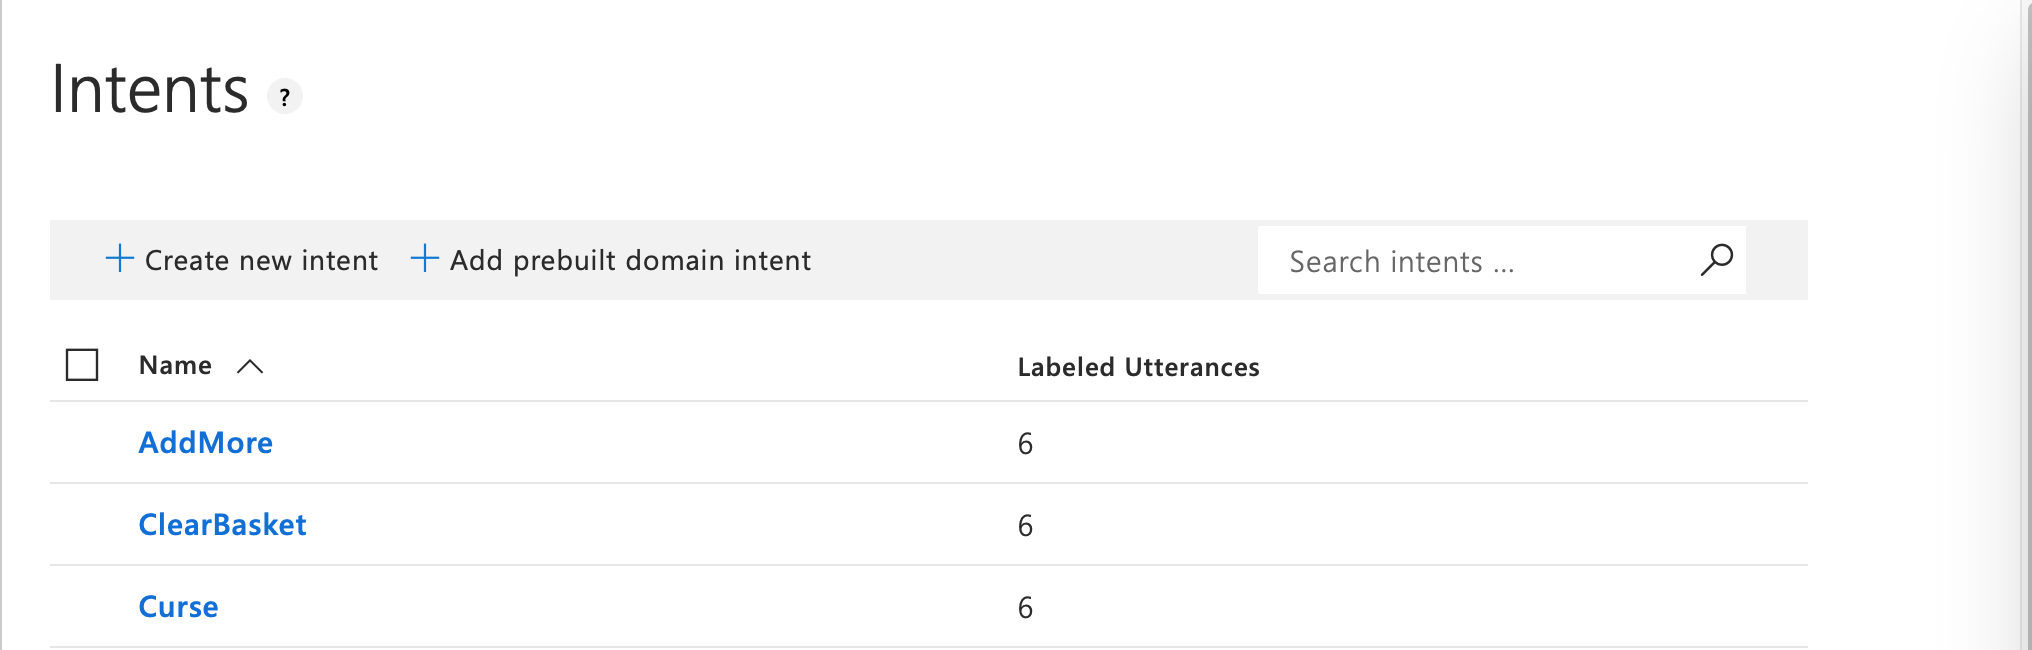
\includegraphics[height=4cm]{img/intents.png}
	\caption{Intent aanmaken Luis.ai}
	\label{fig:intents}
\end{figure}

In de meeste gevallen is een utterance toevoegen niet zomaar eenvoudigweg een zin toevoegen. Meestal zal er in een utterance één of meerdere entities terug te vinden zijn. Bijvoorbeeld in voorgaand voorbeeld bij de intent 'Greeting' konden we een utterance toevoegen 'Hello, I'm Ivor'. In deze utterance is Ivor een entity, namelijk een naam. Het voordeel van deze entities uit de zinnen te halen, is dat bijvoorbeeld de chatbot dan al direct weet dat 'Ivor' de naam is van de persoon die communiceert met de bot en kan de bot deze persoon aanspreken met zijn naam. Dit maakt het gesprek al persoonlijker.

LUIS heeft zelf al een redelijk aantal ingebouwde entities, zoals nummers, leeftijden, e-mail adressen, ... en kan deze makkelijk zelf al herkennen. Indien er geen ingebouwde entity bestaat kan er zelf een entity aangemaakt worden en deze makkelijk linken aan het juiste woord in een utterance.

\begin{figure}[h!]
	\centering
	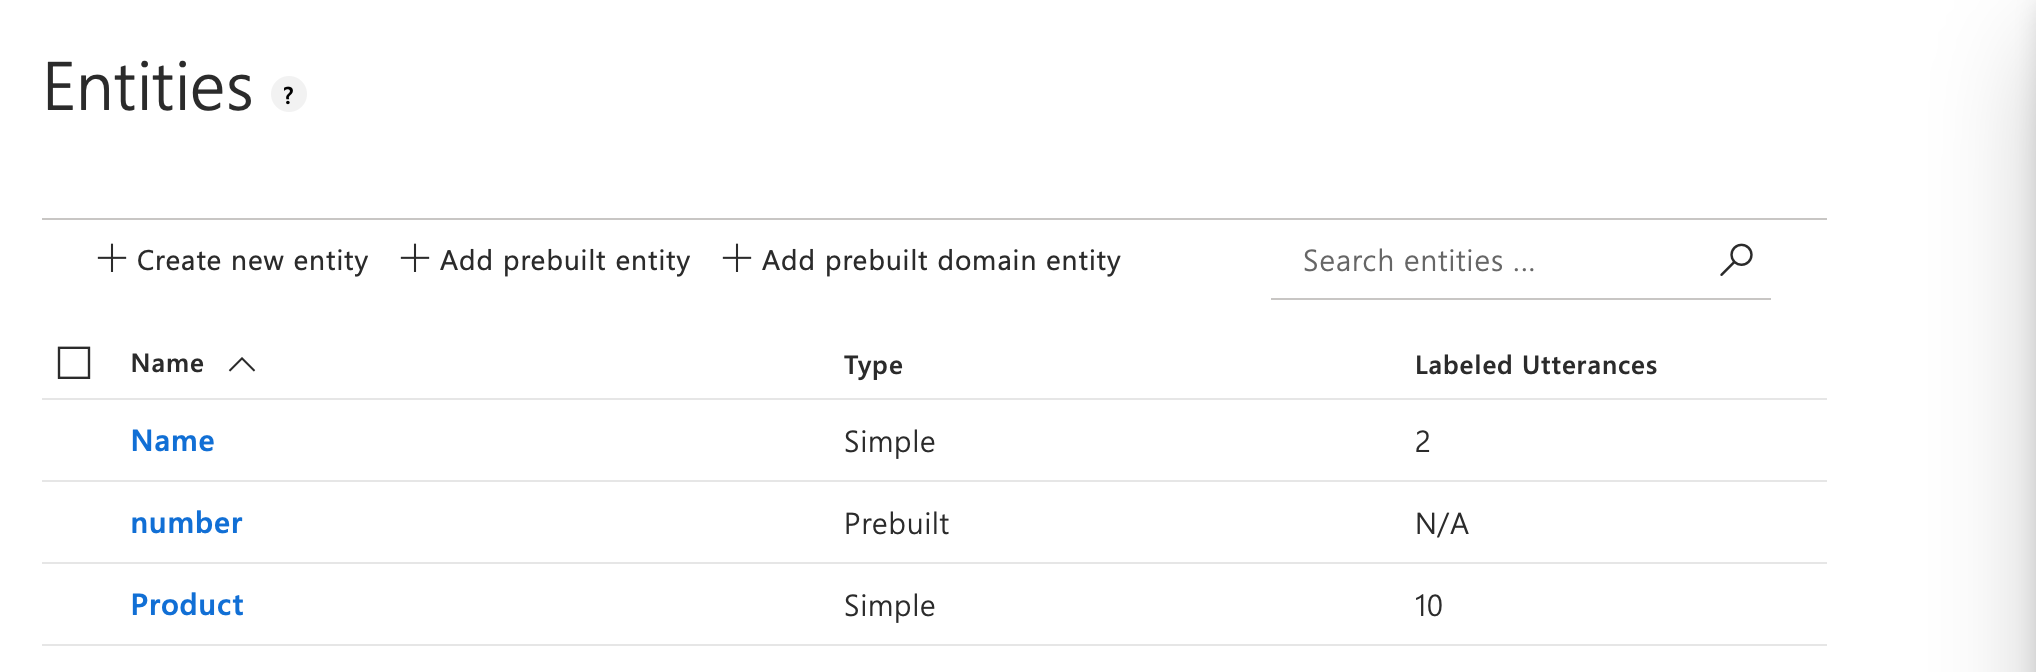
\includegraphics[height=4cm]{img/entity.png}
	\caption{Entities aanmaken Luis.ai}
	\label{fig:entity}
\end{figure}

Eenmaal er enkele intents aangemaakt zijn en bij elke intent enkele utterances zijn toegevoegd (het is aangeraden van er minimum 5 toe te voegen voor een betere accuraatheid) met daarbij eventueel de gepaste entities kan de chatbot als eens getest worden.

Het enige dat nog moet gebeuren vooraleer er kan getest worden, is LUIS trainen. Na het toevoegen van nieuwe intents, entities en utterances dient LUIS opnieuw getraind te worden met de nieuwe data. Na enkele seconden trainen staat alles klaar om getest te worden.

Op de site van LUIS zelf kan er gepraat worden met de chatbot via een simpele interface. Hierin kan er simpelweg gepraat worden met de bot door utterances in te geven. Als voorbeeld kan er weer gebruik worden gemaakt van de utterance: 'Hi, I'm Ivor'. Zo kan er gezien worden of deze de juiste intent herkent en de entity er juist uithaalt met daarbij het percentage van de zekerheid dat LUIS juist is. Bij dit voorbeeld is LUIS er 81 percent zeker van dat deze utterance hoort bij de intent 'Greeting' met de entity 'Ivor' als 'name'.

Indien de utterance niet hoort bij de door LUIS geselecteerde intent kan deze handmatig aangepast worden naar de correcte en kan LUIS opnieuw getraind worden zodat dit de volgende keer correct is.

\begin{figure}[h!]
	\centering
	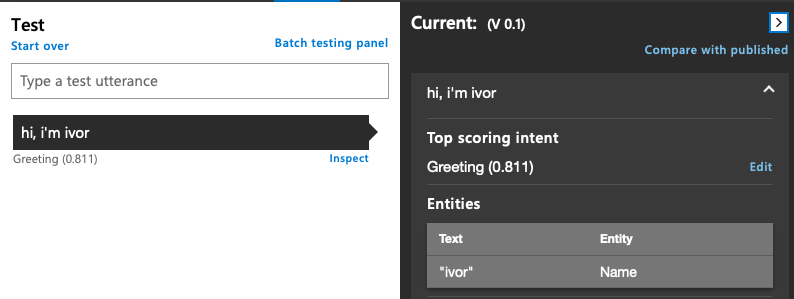
\includegraphics[height=4cm]{img/test.png}
	\caption{Testen van de chatbot Luis.ai}
	\label{fig:test}
\end{figure}

Als alles goed verloopt en bij het testen zijn er niet veel fouten, kan de applicatie gepubliceerd worden. Dit zorgt ervoor dat er vanuit een eigen applicatie een chatbot kan geïntegreerd worden.

Eenmaal deze geïntegreerd is in een eigen applicatie kan er lokaal getest worden op wat de chatbot reageert op bepaalde utterances. Dit kan makkelijk getest worden via de 'Bot Framework Emulator'. Dit is een zeer handig applicatie voor het testen van de bot. Er is een interface zodat het direct lijkt op een echt chatvenster. Hiernaast is er ook een inspector. Hierin komen alle GET en POST boodschappen die worden gestuurd en ontvangen. Zo kan er makkelijk gezien worden als er iets is misgelopen.

\begin{figure}[h!]
	\centering
	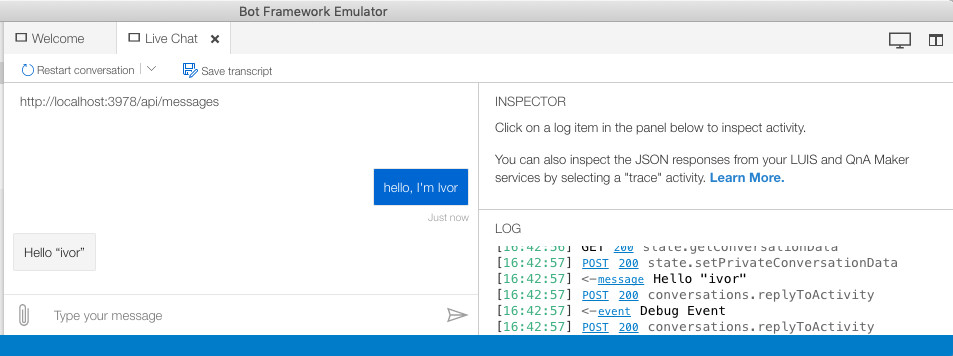
\includegraphics[height=4cm]{img/emulator.png}
	\caption{Bot Framework Emulator}
	\label{fig:emulator}
\end{figure}

Als de LUIS-applicatie gepubliceerd is en deze ontvangt input van gebruikers door bijvoorbeeld via de Bot Framework Emulator, analyseert LUIS elk van deze utterances. LUIS probeert die dan te linken aan de juiste intent. LUIS zal nooit 100 percent zeker zijn dat een bepaalde utterance behoort tot één specifieke intent. LUIS zal de utterances die de gebruiker invoert waar hij niet zo zeker van is, verzamelen onder 'Review endpoint utterances'. Onder deze pagina bevinden zich alle utterances waar LUIS minder zeker van is zodat deze manueel kunnen gelinkt worden aan de juiste intent, utterance per utterance. Bij elke utterance geeft LUIS zelf al een schatting bij welke intent deze hoort. Afbeelding \ref{fig:review} toont de schattingen van LUIS aan de hand van het percentage dat hij zeker is dat de utterance bij een bepaalde intent hoort. Als deze juist is, kan deze toegevoegd worden. 

Indien dit niet juist is, kan er via een dropdown menu de juiste intent geselecteerd worden en deze dan handmatig toevoegen. Bij deze dropdown staan alle intents in volgorde van zekerheid met het percentage erbij. Bij dit voorbeeld 'Let's add 3 more' is de gesuggereerde intent van LUIS AddMore met een percentage van 89.2 percent. De tweede suggestie is FintItem met een percentage van 1.8 percent. Door het grote verschil aan percentages wordt er niet getwijfeld dat deze utterance hoort bij de intent 'AddMore'. De entities van elk van deze utterances worden door LUIS automatisch gedetecteerd. Moest het zijn dat LUIS dat niet gedaan heeft, kunnen de entities handmatig aangeduid worden.

\begin{figure}[h!]
	\centering
	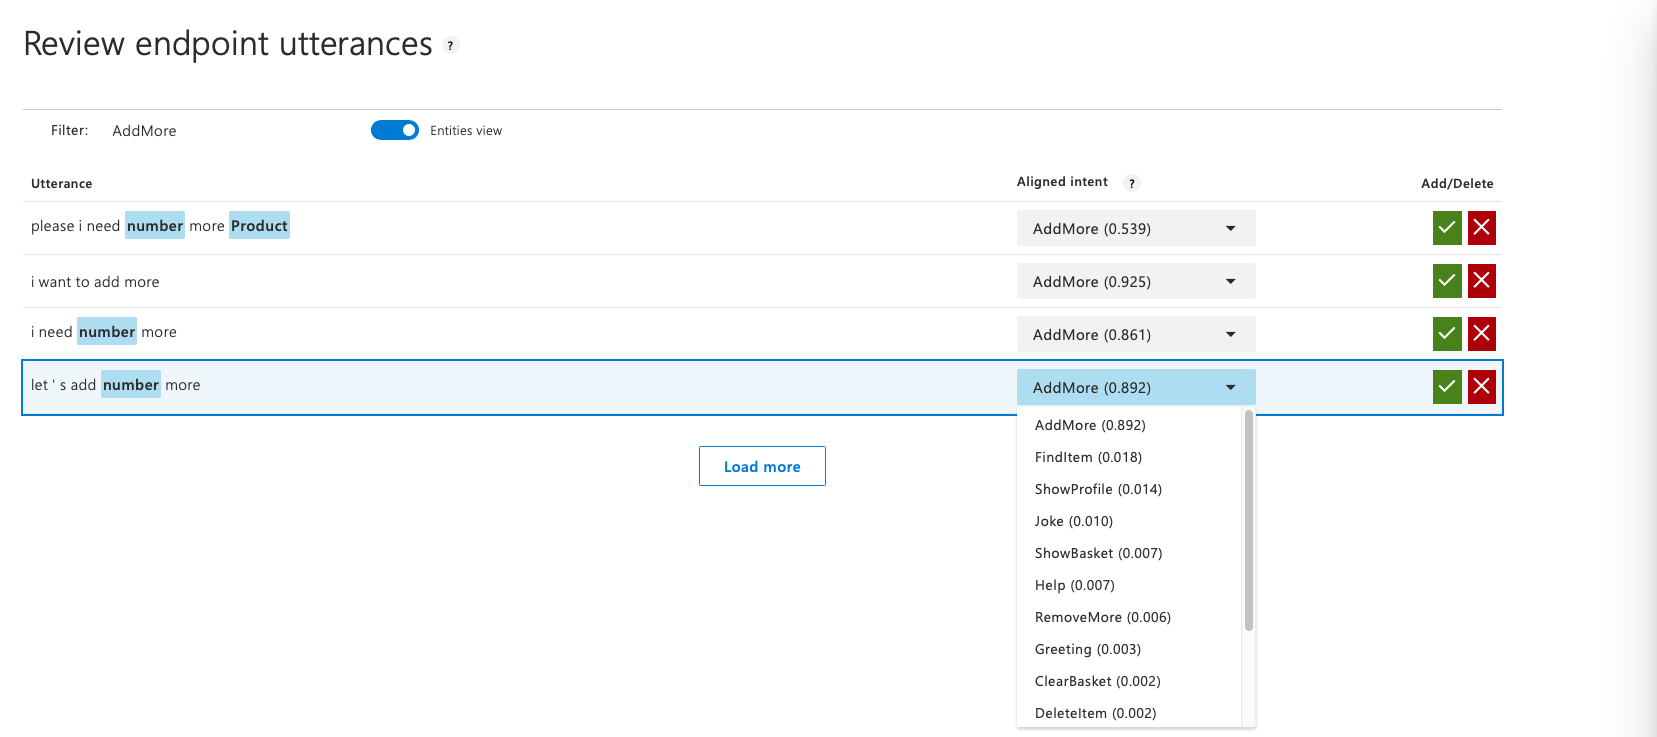
\includegraphics[height=6cm]{img/review.png}
	\caption{Review endpoint utterances Luis.ai}
	\label{fig:review}
\end{figure}

Dit was een zeer goed begin om te begrijpen wat de concepten zijn van een framework voor het ontwikkelen van chatbots. Door het op voorhand bestuderen van één bepaald framework voor het maken van chatbots worden al veel aspecten zeer duidelijk en deze zijn meestal wel hetzelfde voor de andere frameworks ook. Door LUIS al eens te bestuderen is het doel van deze bachelorproef direct veel duidelijker geworden. De review endpoint utterances uit afbeelding \ref{fig:review} dient nu allemaal handmatig te worden goedgekeurd en nagekeken. Zoals er kan gezien worden, is het niet nodig om bij elke utterance handmatige controle te steken. Soms is de score van de eerste en de tweede gesuggereerde intent zo groot dat er geen twijfel mogelijk is bij welke intent deze behoort. Bij alle utterances waarbij dit het geval is, zou deze handmatige controle achterwege kunnen worden gelaten.

In het volgende deel worden verschillende van de bekendste frameworks voor het maken van bot vergeleken. Hierbij zal gekeken worden of deze een API hebben en of deze toegankelijk genoeg is voor de 'review endpoint utterances' op te halen en deze via een API-call op te halen in een eigen applicatie, deze automatisch te controleren en goedkeuren indien dit kan. Zo zullen uiteindelijk de utterances die nog handmatig zullen moeten gecontroleerd worden veel minder zijn.

Nu dat de basisconcepten van LUIS duidelijk zijn, kan er worden gekeken of LUIS een API heeft en of deze toegankelijk genoeg is voor de onderzoeksvraag te kunnen oplossen. Al snel is duidelijk dat er effectief een API bestaat genaamd 'LUIS Programmatic APIs v2.0'. Hierin is er een grote variatie, van het toevoegen van intents en entities naar het toevoegen van een nieuwe utterance en meer. Voor het ophalen van utterances is er één API-call 'Review labeled examples'. Deze call heeft enkel de utterances weer die al zijn toegevoegd aan een bepaalde intent, dus jammer genoeg niet de 'unlabeled examples'. De utterances waarvan LUIS niet exact weet bij welke intent deze hoort, die op de site van LUIS zelf onder 'review endpoint utterances' staan, kunnen niet worden opgehaald via een API-call en kunnen dus niet automatisch gecontroleerd worden.

\subsection{Wit.ai}
\label{Wit}

Wit.ai hoort ook bij één van de bekendste frameworks voor het ontwikkelen van chatbots. De grote lijnen van dit framework zijn wat hetzelfde als die van LUIS.

Eerst en vooral moet er een applicatie worden aangemaakt met de naam, de taal waarin de bot zal functioneren en eventueel een omschrijving. Het toevoegen van intents en utterances werkt op een verschillende manier maar komt uiteindelijk op hetzelfde neer. Afbeelding \ref{fig:intentsWit} toont hoe dit in zijn werk gaat. Hier moet er begonnen worden met het invoeren van een utterance en dan kunnen deze gelinkt worden met een intent. Hier kunnen we weer het voorbeeld gebruiken van 'Hi, I'm Ivor'.

\begin{figure}[h!]
	\centering
	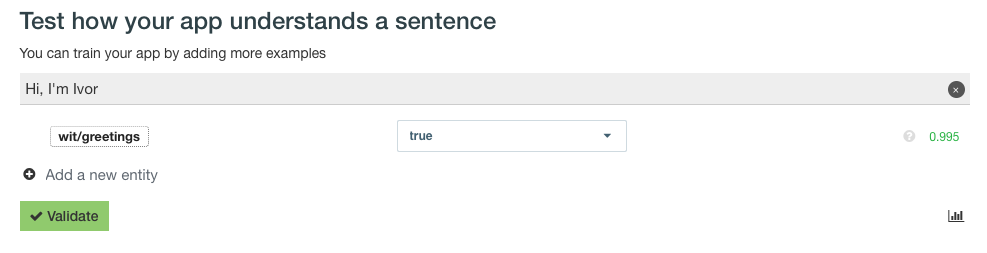
\includegraphics[height=4cm]{img/wit_intents.png}
	\caption{Intent aanmaken Wit.ai}
	\label{fig:intentsWit}
\end{figure}

Wit herkent dit al automatisch als een 'Greeting', hier wordt ook het percentage van 99 percent gezien. Dit percentage is zoals bij LUIS de zekerheid dat Wit denkt dat een intent bij een bepaalde utterance hoort. Indien Wit deze niet herkent of de intent bestaat simpelweg nog niet, kan deze hier aangemaakt en toegevoegd worden. Dit werkt juist op dezelfde manier bij het toevoegen van een entity.

Het weergeven van de al ingevoerde utterances verschilt ook van LUIS. In Wit is er een tabblad 'Samples' waarbij alle utterances worden getoond onder elkaar. Hier kunnen de utterances gefilterd worden per intent.

\begin{figure}[h!]
	\centering
	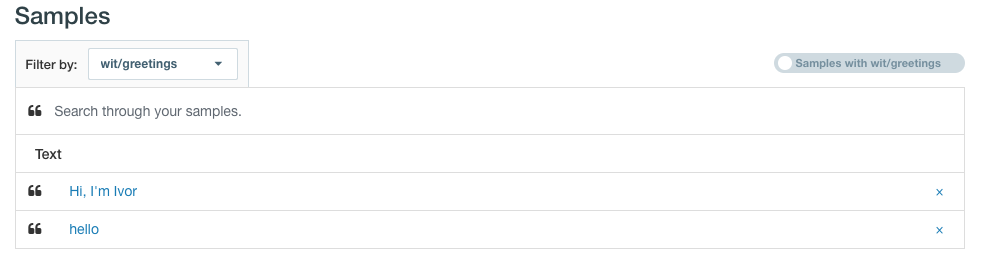
\includegraphics[height=4cm]{img/samples.png}
	\caption{Utterances toevoegen Wit.ai}
	\label{fig:samples}
\end{figure}

Ook heeft Wit net zoals LUIS een pagina waar de utterances inkomen van de gebruikers die praten met de bot waarvan Wit niet exact weet bij welke intent deze horen. Hierin suggereert Wit ook aan de hand van een percentage bij welke intent hij denkt dat een bepaalde utterance hoort. Deze kunnen dan ook nagekeken worden of alles klopt. Indien dit niet juist is, kan deze veranderd worden via de dropdown en deze dan gevalideerd worden. De gevalideerde utterance wordt daarna toegevoegd aan de lijst van de samples met zijn intent.

Ook bij Wit zouden deze reviews moeten worden geautomatiseerd. Nu de basiswerking van Wit duidelijk is geworden, kan er worden gekeken naar de toegankelijkheid van de API. 

\begin{figure}[h!]
	\centering
	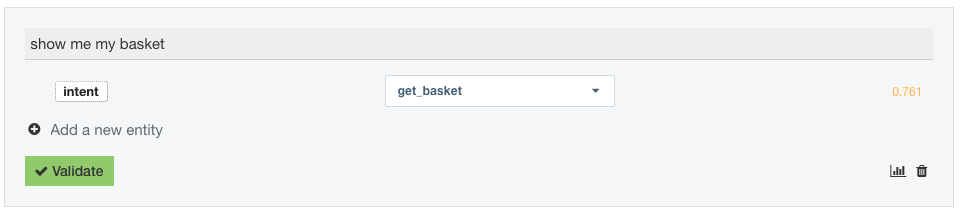
\includegraphics[height=3.5cm]{img/inbox.png}
	\caption{Valideren ongelabelde utterances Wit.ai}
	\label{fig:inbox}
\end{figure}

Wit heeft ook wel degelijk een API ter beschikking. De API lijkt zeer sterk op deze van LUIS, er kunnen nieuwe utterances aan worden toegevoegd, samen met nieuwe intent en entities. Ook kunnen hier de utterances worden opgehaald die al gelinkt zijn aan een bepaalde intent. Net zoals bij LUIS zijn de utterances waarvan Wit niet zeker weet bij welke intent ze horen hier niet bij. Deze zullen dus via de webpagina zelf moeten gevalideerd worden en zal niet automatisch kunnen worden gecontroleerd.

\subsection{IBM Watson Assistant}
\label{watson}

Een derde framework voor het bouwen van chatbots is IBM Watson Assistant. Dit framework werkt ook gedeeltelijk op een andere manier dan de vorige onderzochte frameworks. Voor het ontwikkelen van een chatbot in IMB Watson Assistant zijn er drie grote stappen.

De eerste stap is het maken van een 'Skill'. Onder de skill bevindt zich alle logica van de bot, de bot wordt hier getraind. Een skill kan hier vergeleken worden met een App dat eerst moet worden gemaakt bij de vorige frameworks. Eerst en vooral dient een skill te worden aangemaakt. Een skill heeft een naam, de taal waarin tegen de bot zal gesproken worden en eventueel een omschrijving. Eenmaal deze skill is aangemaakt, kunnen er zeer eenvoudig intents worden aangemaakt en aan elke intent utterances worden toegevoegd.

\begin{figure}[h!]
	\centering
	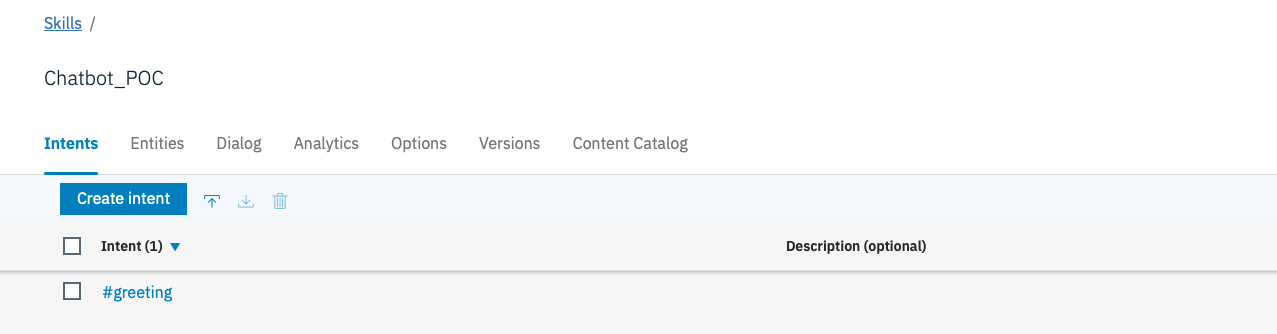
\includegraphics[height=4cm]{img/ibm_intents.png}
	\caption{Intent aanmaken IBM Watson Assistant}
	\label{fig:intentsIbm}
\end{figure}

Na het aanmaken van een bepaalde intent wordt er naar de detailpagina van deze intent genavigeerd. Op deze pagina kunnen utterances worden toegevoegd aan deze intent. De werking van dit toevoegen lijkt zeer sterk op die van LUIS. Een entity kan hier ook zeer makkelijk aangeduid worden door de gewenste woorden te selecteren en de juiste entity aan te klikken. Indien de entity nog niet bestaat, kan deze hier even snel direct worden aangemaakt en toegewezen.

\begin{figure}[h!]
	\centering
	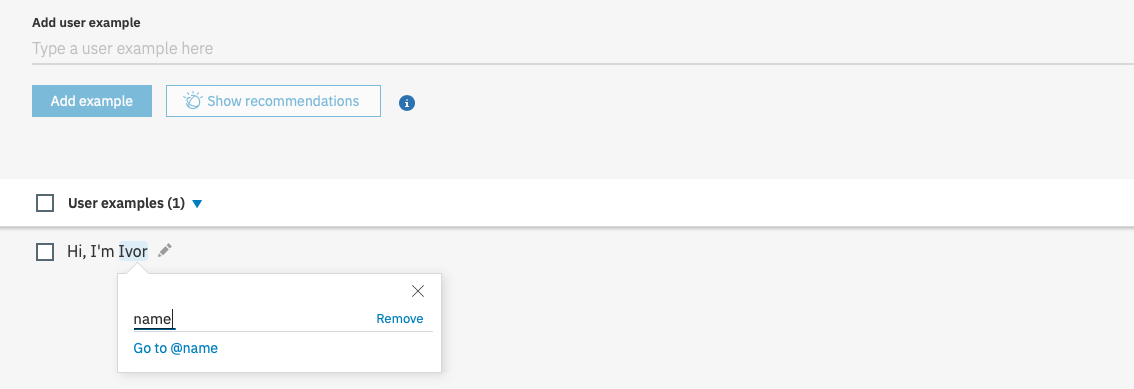
\includegraphics[height=4cm]{img/imb_utterances.png}
	\caption{Utterances toevoegen IBM Watson Assistant}
	\label{fig:utterancesIbm}
\end{figure}

Het trainen van de Skill gaat hier vanzelf. Daarna kan de bot al eens getest worden met de al toegevoegde intents en entiteiten. Als voorbeeld kan er weer worden ingegeven 'Hi, I'm Ivor'. Er kan al direct worden gezien aan welke intent de utterance wordt gelinkt. In vergelijking met LUIS en Wit zijn er hier bij het testen geen percentages. Er is dus niet geweten hoeveel percent de Skill zeker is van een bepaalde intent. Ook kan er direct gezien worden welke entities er worden herkend. Dit wordt getoond in figuur \ref{fig:tryIbm}.

\begin{figure}[h!]
	\centering
	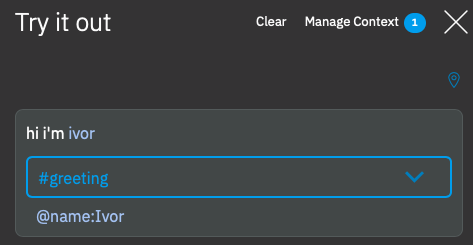
\includegraphics[height=4cm]{img/ibm_try.png}
	\caption{Testen van de Skill IBM Watson Assistant}
	\label{fig:tryIbm}
\end{figure}

De tweede stap in dit proces is het deployen van de skill met een assistant. In deze stap wordt de skill aan een assistant gelinkt. Hierin is het eerst nodig om een nieuw assistant te maken. Alleen een naam is vereist, een beschrijving is optioneel. Eenmaal de assistant is gecreëerd, kan er een skill worden aan toegevoegd. Daarna kan er een kanaal worden gekozen waarop de bot kan worden gedeployed. Hierbij is er ook een preview waarop kan worden getest.

De utterances waarvan de assistant niet zeker is bij welke intent deze horen, worden bijgehouden en kunnen teruggevonden worden onder het tabblad 'Analytics'. Hier kan er worden doorgeklikt naar de 'Weak understandings'. Hierin kunnen de utterances worden gelinkt aan de juiste intent. Wat verschillend is met vorige frameworks is dat de assistant geen enkele intent aanbeveelt aan de hand van scores. Hier moet er 100 percent zelf worden nagedacht bij welke intent deze hoort.

\begin{figure}[h!]
	\centering
	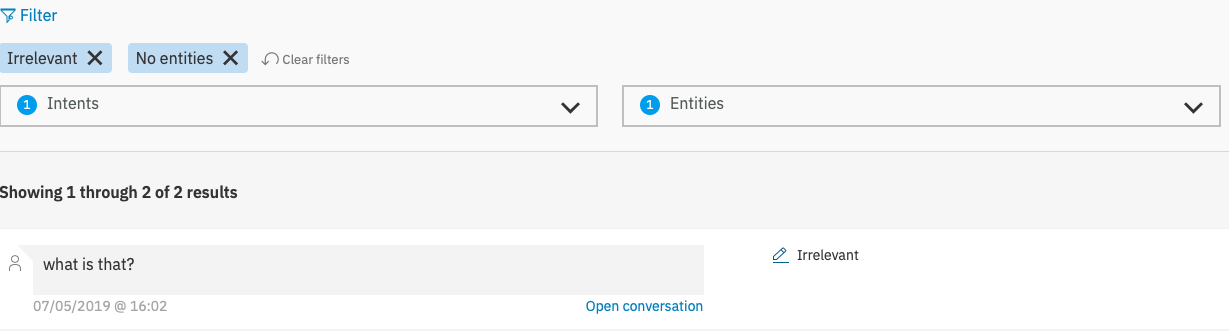
\includegraphics[height=4cm]{img/weak.png}
	\caption{Weak understandings IBM Watson Assistant}
	\label{fig:weak}
\end{figure}

IBM Watson Assistant heeft ook een API. Deze API is zeer uitgebreid en bevat zo goed als alle aspecten van de site zelf. Van het creëren van een intent tot het toevoegen van nieuwe utterances en veel meer. In vergelijking met vorige frameworks heeft de assistant van IBM ook een endpoint voor het ophalen van utterances waarvan de assistant niet zeker is. Het enige probleem hier is dat IBM geen scores voorziet bij een utterance, dus zal er altijd manuele controle nodig zijn. De niet-gelinkte utterances kunnen hier wel opgehaald worden met een eigen applicatie maar de scores ontbreken, dus zal er niet automatisch kunnen gecontroleerd worden of deze utterance is gelinkt met de juiste intent.

\subsection{Dialogflow}
\label{dialogflow}

Dialogflow is een chatbot-framework gemaakt door Google. Net zoals de vorige frameworks is er hier de mogelijkheid om op een relatief eenvoudige manier een chatbot op te zetten. Hierbij is de eerste stap om een 'Agent' te maken. Dit wordt gedaan door de naam van de Agent, de taal die er zal worden gesproken tegen de bot en de tijdzone in te geven.

Een intent aanmaken is hier ook zeer eenvoudig, dit kan door de naam van de intent in te geven. Daarna kunnen er al direct utterances aan toegevoegd worden bij 'Training phrases' zoals er wordt getoond in afbeelding \ref{fig:intentsdialogflow}. De entities kunnen ook toegevoegd worden aan de intent door deze te selecteren en de juiste entity te kiezen. Hierbij zijn er al een aantal ingebouwde entities voorzien. Indien de entity niet in de lijst staat, kan er een nieuwe worden aangemaakt in het 'Entities' tabblad, dit kan eenvoudigweg door de naam van de entity in te vullen.

\begin{figure}[h!]
	\centering
	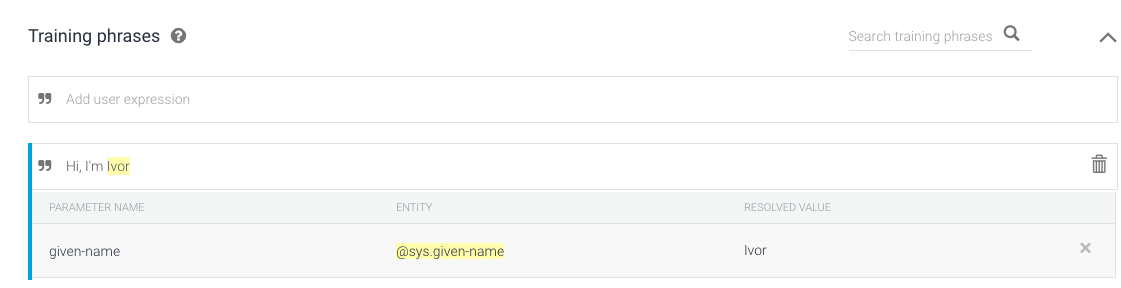
\includegraphics[height=4cm]{img/dialogflow_intents.png}
	\caption{Intent aanmaken Dialogflow}
	\label{fig:intentsdialogflow}
\end{figure}

Deze gemaakte intents met de toepasselijk toegevoegde utterances kunnen al direct getest worden door de console die is voorzien. Er kan als voorbeeld 'Hi, I'm Ivor' gebruikt worden. Hierin kan gezien worden op afbeelding \ref{fig:testdialogflow} dat deze input wordt geanalyseerd door de bot. Deze ziet dat de voorbeeldzin past bij de juiste intent 'Greeting' en dat de waarde 'Ivor' een entity is.

\begin{figure}[h!]
	\centering
	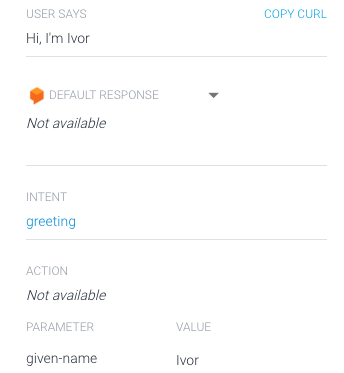
\includegraphics[height=6cm]{img/dia_test.png}
	\caption{Valideren ongelabelde utterances Dialogflow}
	\label{fig:testdialogflow}
\end{figure}

Bij dialogflow is er ook de kans om de utterances die de gebruiker ingeeft waarvan de bot niet zeker is bij welke intent deze horen te bekijken en te valideren. Hier is er zowat hetzelfde probleem als bij de IBM Watson Assistant, als dialogflow echt niet zeker is van de intent zal er in de testconsole de intent 'default failback intent' komen. Bij het training tabblad dient er dan zelf te worden gekeken welke intent hier dan exact bij hoort en dialogflow zal niet suggereren wie welke deze hoort. Er zijn hier ook geen percentages, dus er kan niet worden gezien waaraan dialogflow een bepaalde utterance zou linken die niet direct herkend wordt.

\begin{figure}[h!]
	\centering
	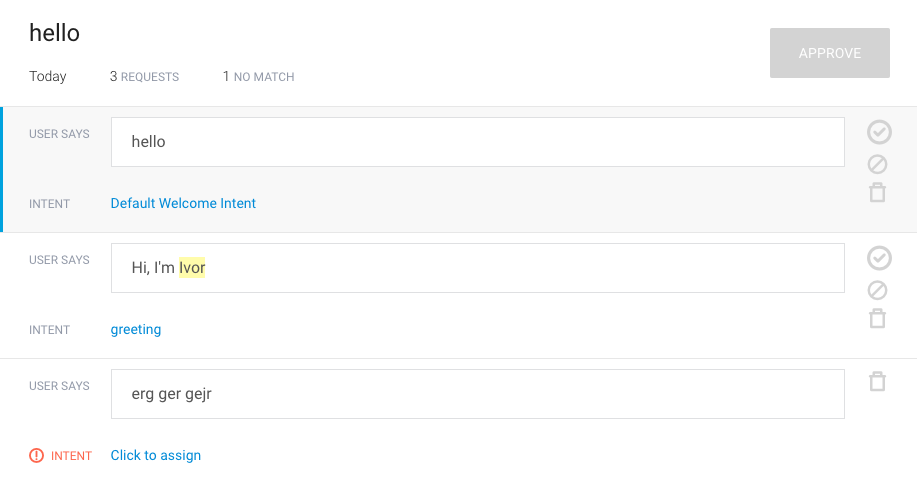
\includegraphics[height=6cm]{img/dia_training.png}
	\caption{Utterances toevoegen Dialogflow}
	\label{fig:trainingdialogflow}
\end{figure}

Dialogflow heeft ook een API. Deze kan zogoed als enkel het noodzakelijkste, zoals intent en entities aanmaken en utterances toevoegen en nog enkele zaken. Via de API kunnen de utterances van de gebruikers waarvan dialogflow niet weet bij welke intent die past niet opgevraagd worden. Deze kunnen dus niet worden geïntegreerd in een eigen applicatie om die automatisch bij de juiste intent toe te wijzen. Ook zou hier nog een ander probleem zijn zoals bij IBM Watson Assistant dat er geen percentages worden weergegeven. Moest er zelf een API voor zijn om deze op te halen, zouden ze niet automatisch kunnen toegewezen worden door het gebrek aan deze percentages van zekerheid.

\subsection{Andere frameworks}
\label{andereFrameworks}

Verder zijn er nog een aantal frameworks bekeken en vergeleken zoals Amazon Lex, BotKit, BotPress, BotMan, Rasa Stack, SAP Conversational AI, enz. Al snel was er ingezien dat deze frameworks dezelfde problemen met zich mee brachten zoals de al vergeleken frameworks ofwel hadden deze frameworks geen API die kon worden gebruikt. 

\subsection{Conclusie frameworks}
\label{conclusieFrameworks}

Bij geen enkel van de onderzochte frameworks is het mogelijk om via de API de utterances op te halen waarvan het framework niet zo goed weet of hij ze gelinkt heeft aan de correcte intent. Om dan zo via deze API-call al deze utterances op te halen en te verwerken in een eigen applicatie, die er dan voor zorgt dat deze automatisch worden gecontroleerd en gelinkt worden aan de juiste intent, enkel als de zekerheid groot genoeg is. Als de zekerheid niet goed is, met andere woorden als de applicatie twijfelt tussen 2 intents omdat de percentages van deze veel te dicht bij elkaar liggen, zal er niets gedaan worden en zal deze handmatig moeten worden gecontroleerd. Eenmaal gecontroleerd zou de utterance via een andere API-call kunnen toegevoegd worden aan de juiste intent in het framework zelf. Zo zouden maar een beperkt aantal van de utterances handmatig moeten gecontroleerd worden doordat er al veel automatisch worden verwerkt.

Dit alles is niet mogelijk door de beperkingen van de API's van deze frameworks of doordat er geen scores (percentages) worden meegeleverd met de API-call.

Er is echter wel een manier om dit alles mogelijk te maken door het op een andere manier aan te pakken. Namelijk door alle input van gebruikers op te vangen in een eigen applicatie, deze input daarna door te sturen naar de bot zelf en de resultaten opvangen. Hierin wordt gezien welke intents er aan deze utterance gelinkt worden met een percentage erbij. Bijvoorbeeld als er 'Hello' wordt gestuurd, zullen er een paar intents worden teruggegeven. Hier bijvoorbeeld 'Greeting' met een percentage van 92 percent en 'Curse' met een percentage van 3 percent. Deze percentages verschillen heel veel. Op deze manier weet de applicatie dan direct dat hello bij de intent 'Greeting' hoort en zal deze utterance toevoegen aan deze intent. Indien de applicatie niet zeker is en de 2 percentages liggen te dicht bij elkaar of zijn beide veel te laag, zal deze niet toegevoegd worden en zal deze utterance automatisch worden toegevoegd aan de lijst van de utterances waarvan de bot niet zeker is.

Het werken op deze manier zal uiteindelijk dezelfde resultaten bekomen. De utterances die dan worden geanalyseerd en uiteindelijk worden toegevoegd, zullen niet meer in de lijst komen van utterances waarvan de bot niet zeker is. Dat is uiteindelijk de bedoeling van het uitwerken van de onderzoekvraag. De input van de gebruiker zal gedeeltelijk automatisch worden toegevoegd aan de juiste intent maar niet allemaal. Er zijn altijd utterances waarvan de chatbot geen goede suggesties kan weergeven en die zullen dan handmatig moeten worden toegevoegd. Hoe meer utterances per intent, hoe beter die suggesties zullen zijn. Dus hoe langer de chatbot in productie zou zijn, hoe minder utterances er handmatig zouden moeten worden gecontroleerd.



\definecolor{lightgray}{rgb}{.9,.9,.9}
\definecolor{darkgray}{rgb}{.4,.4,.4}
\definecolor{purple}{rgb}{0.65, 0.12, 0.82}

\lstdefinelanguage{JavaScript}{
	keywords={typeof, new, true, false, catch, function, return, null, catch, switch, var, if, in, while, do, else, case, break},
	keywordstyle=\color{blue}\bfseries,
	ndkeywords={class, export, boolean, throw, implements, import, this},
	ndkeywordstyle=\color{darkgray}\bfseries,
	identifierstyle=\color{black},
	sensitive=false,
	comment=[l]{//},
	morecomment=[s]{/*}{*/},
	commentstyle=\color{purple}\ttfamily,
	stringstyle=\color{red}\ttfamily,
	morestring=[b]',
	morestring=[b]"
}

\lstset{
	language=JavaScript,
	backgroundcolor=\color{lightgray},
	extendedchars=true,
	basicstyle=\footnotesize\ttfamily,
	showstringspaces=false,
	showspaces=false,
	numbers=left,
	numberstyle=\footnotesize,
	numbersep=9pt,
	tabsize=2,
	breaklines=true,
	showtabs=false,
	captionpos=b
}

\chapter{\IfLanguageName{dutch}{Proof of concept}{Proof of concept}}
\label{ch:poc}

In dit onderdeel zal de proof of concept besproken worden. In deze proof of concept wordt er gebruikgemaakt van de Microsoft bot framework SDK en van LUIS.

\section{Gekozen framework}
\label{sec:framework}

Uit het onderzoek is gebleken dat LUIS de juiste keuze is uit alle vergeleken frameworks voor het maken van bots. Het is belangrijk dat de API een goede toegankelijkheid heeft en dat er per weergegeven utterance informatie is over de verschillende intents en daarbij een percentage.

Door de goede toegankelijkheid van de API is er een mogelijkheid om de interface van LUIS zelf achterwege te laten en LUIS bijna volledig in een eigen applicatie te kunnen implementeren, zoals het toevoegen van intents, entities, utterances. Het enige dat niet kan worden opgehaald zijn de 'review endpoint utterances'. Maar juist door de goede toegankelijkheid kan dit op een andere manier worden opgelost, besproken in de conclusie van vorige hoofdstuk.

Doordat LUIS bij elke utterance veel info teruggeeft over de intents waarbij deze kunnen behoren met daarbij dan nog eens de percentages van zekerheid dat een utterance bij een intent hoort, kan er worden gekeken hoezeer LUIS zeker is dat een utterance bij die bepaalde intent hoort.

Dat zijn de belangrijkste zaken waarmee er rekening moet gehouden worden voor de onderzoeksvraag te kunnen uitwerken. In dit geval is er één van de frameworks daartoe instaat om deze zaken te garanderen. Wit.ai en IBM Watson kwamen in de buurt maar ze voorzien niet genoeg informatie bij elke utterance. Er wordt wel gebruikgemaakt van scores bij Wit maar bij elke utterance is er maar 1 intent met score voorzien in vergelijking met LUIS waarbij alle intents worden gezien met de score daarbij. Bij IBM Watson kunnen de utterances die nog niet gevalideerd zijn worden opgehaald via een API maar hier zijn totaal geen scores bij inbegrepen.

Ook komt dit goed uit dat LUIS wordt gekozen als framework dat dit kan realiseren omdat de opdrachtgever Endare, zelf ook gebruik maakt van LUIS voor het ontwikkelen van chatbots en zijn daarmee het meest vertrouwd.

\section{Opzetten LUIS}
\label{sec:opzet}

Voor de opzet van de LUIS intents en utterances is er mij een voorbeeld toegereikt van de opdrachtgever Endare, zodat het model niet van nul zou moeten worden begonnen. Vanaf dit voorbeeld kan er verder gewerkt worden door nieuwe intents toe te voegen zodat deze alsmaar beter wordt.

LUIS zal hier worden getraind als een soort van hulp bij de aankoop van producten en onderhoud en weergave van het account en winkelmandje. Zo kunnen er bijvoorbeeld producten worden toegevoegd aan het mandje, ook de producten kunnen verwijderd worden, producten zoeken, hulp inroepen, het mandje tonen en verwijderen, het profiel tonen en aanpassen zijn ook allemaal mogelijk.

\begin{figure}[h!]
	\centering
	
\includegraphics[height=10cm]{img/luis.png}
	\caption{Overzicht intents Luis.ai}
	\label{fig:trainingdialogflow}
\end{figure}

De intents die zijn toegevoegd zijn: AddMore, ClearBasket, Curse, DeleteItem, FindItem, Greeting, Help, Joke, RemoveMore, ShowBasket, ShowProfile, Stop en UpdateProfile. Bij elke intent zijn er ongeveer 5 tot 10 utterances toegevoegd, wat al een goed begin is voor het correct trainen van de bot.

De entities die zich in LUIS bevinden zijn name, number en product waarvan number een ingebouwde entity is en de andere twee zelf gemaakte entities zijn. De naam dient als aanspreking bij de 'Greeting' intent. De entity 'number' is voor een hoeveelheid mee te geven bij bijvoorbeeld de intent 'AddMore', zodat er meerdere producten kunnen worden toegevoegd. De entity 'product' is voor te weten over welk product er gesproken wordt.

LUIS is volledig in het Engels geschreven omdat Engels de taal is dat het beste wordt begrepen door LUIS. Dit zal dan ook resulteren in betere resultaten als een gebruiker praat tegen de bot. Indien de bot Nederlands moet verstaan kunnen er twee dingen gebeuren. Ofwel  kan er een andere LUIS applicatie aangemaakt worden volledig in het Nederlands ofwel kan er een middleware worden tussengestoken die de Nederlandse tekst omzet naar het Engels zodat de Engelstalige versie van LUIS alles verstaat. De beste en gemakkelijkste optie is het tweede omdat er ten eerste minder werk zal zijn. Er zal maar 1 LUIS app moeten gemaakt worden, dus enkel in het Engels. Ook zal LUIS beter werken omdat hij Engels beter verstaat dan het Nederlands.

\section{Software}
\label{sec:POC}

\subsection{Node.js en TypeScript}
\label{ts}

De keuze om de applicatie te ontwikkelen met Node.js in TypeScript was niet zo moeilijk. Omdat er bij Endare, het bedrijf die met de onderzoeksvraag is gekomen, wordt gewerkt met Node.js is de keuze snel gemaakt om het met Node.js te maken. Door dit te doen met de gebruikelijke tools van dat bedrijf zorgt er voor eventueel latere implementatie een gebruiksgemak doordat de taal hetzelfde is en niet zal moeten worden omgezet. Daardoor ook de keuze om het in TypeScript te maken in de plaats van JavaScript omdat Endare is overgestapt naar TypeScript.

\subsection{Bot Framework Emulator}
\label{emulator}

Dit is een applicatie gemaakt voor ontwikkelaars voor het te kunnen testen van een chatbot. Met de emulator kan er met de bot gepraat worden via de user interface. Er is ook een inspector en een log waar de verzonden en ontvangen berichten verder in detail kunnen worden bekeken.

Het is zeer eenvoudig om met de bot te verbinden. Als deze lokaal aan het runnen is op een eigen applicatie kan er geconnecteerd worden door enkel het localhost-adres op te geven. Daarna is de emulator klaar om met de bot te praten.

\subsection{Microsoft Bot Framework}
\label{botFramework}

Voor het uitwerken van de proof of concept is ervoor gekozen om het Bot Framework SDK te gebruiken van Microsoft. Dit framework is veel gebruikt bij het ontwikkelen van chatbots omdat deze zeer veel mogelijkheden heeft voor het maken van bots. Deze kan gebruikt worden voor zowel simpele console applicaties tot zeer uitgebreide interfaces. Het Bot Framework SDK gebruikt restify, dat is een bekend framework voor het maken van webservices. Dit wordt hier gebruikt voor de webserver van de bot.

Dit SDK heeft een systeem voor het maken van dialogs, er zijn veel ingebouwde zaken zoals kaarten met daarin knoppen, foto's, enz. Wat heel belangrijk is, is dat er een mogelijkheid bestaat voor het implementeren van AI-frameworks. Wat hier zeker een noodzaak is en waar gebruik van zal gemaakt worden. Dit door LUIS te implementeren in het bot framework SDK.

Het installeren van de bot framework SDK (botbuilder) kan eenvoudig worden gedaan door simpelweg een commando in te geven. Daarna kan er onmiddellijk aan de slag worden gegaan met de botbuilder.

Eerst en vooral dient er een HTTP server gecreëerd te worden. Hierop wordt de bot lokaal gehost zodat deze kan worden getest. De bot kan getest worden, gebruik makende van de Bot Framework Emulator als deze HTTP server draait.

\medskip
\begin{lstlisting}[caption=Creatie van de HTTP server]
// create HTTP server \\
var server = restify.createServer();
server.listen(process.env.port || process.env.PORT || 3978, () => {
	console.log(`Listening... ${server.name}... ${server.url}`);
});
\end{lstlisting}

Met de HTTP server alleen is er nog geen connectie met de botbuilder. Een connectie maken kan ook eenvoudig in enkele lijnen code. Daarna kan  LUIS gekoppeld worden aan deze connectie. Dit wordt gedaan aan de hand van het endpoint dat verkregen wordt wanneer LUIS gedeployed wordt op de site van LUIS zelf. Dan ontstaat er een link naar het endpoint. Deze link wordt best in de environment variables gestoken zodat deze veilig blijft naar de buitenwereld toe. Daarna kan geluisterd worden naar inkomende boodschappen die bijvoorbeeld worden ingegeven in de bot framework emulator. 

\medskip
\begin{lstlisting}[caption=Connectie en linken van LUIS]
// connection \\
var conn = new builder.ChatConnector({
	appId: process.env.MICROSOFT_APP_ID,
	appPassword: process.env.MICROSOFT_APP_PASSWORD
});

// link LUIS to botbuilder \\
var bot = new builder.UniversalBot(conn);
bot.recognizer(new builder.LuisRecognizer(process.env.LUIS_MODEL_URL));


// listen for incoming requests \\
server.post("/api/messages", conn.listen());
\end{lstlisting}

Als al deze stappen gedaan zijn, is alles in gereedheid gebracht voor het kunnen verwerken van een bepaalde input. Dit wordt gedaan door dialogs. Aan de hand van de intent die teruggekregen wordt van LUIS voor een bepaalde input van een gebruiker, wordt telkens een andere dialog aangeroepen zodat de juiste actie kan worden ondernomen en het juiste resultaat kan worden teruggegeven.

Een dialog werkt volgens de watervalmethode. Dit betekent dat een dialog van functie naar functie kan gaan. Dit is zodat als eerst dit stukje code en dan dat stukje code als dat eerst gedaan is, enz. Zoals er kan gezien worden in Listing 4.3 wordt er eerst gevraagd naar de naam van de gebruiker. Als de gebruiker deze naam heeft ingegeven, gaat er via de watervalmethode naar de volgende functie gegaan worden waarbij de naam van de gebruiker wordt opgeslagen zodat de bot de naam blijft onthouden voor in de toekomst en wordt er een antwoord teruggestuurd naar de gebruiker.

Dit is een eenvoudig voorbeeld, er kan hierin veel verder worden gegaan, er kan bijvoorbeeld in een dialog een andere dialog aangeroepen worden. Als de naam bijvoorbeeld nog niet geweten is, kan er een dialog worden aangeroepen met als doel de naam van de gebruiker op te vragen maar indien deze wel al geweten is, kan er gewoon verder worden gegaan met de volgende stap in de waterval.

\medskip
\begin{lstlisting}[caption=Watervalmethode]
// dialog \\
bot.dialog("/", [
	function (sess, args, next) {
		if (!sess.userData.name) {
			builder.Prompts.text(sess, "Hello, user! What is your name?");
		}
		else {
			next();
		}
	},
	function (sess, result) {
		sess.userData.name = result.response;
		sess.send("Hello, " + sess.userData.name);
	}
]);
\end{lstlisting}

Dit is zowat de basis van de werking van de botbuilder. Er zijn hier dus nog veel meer mogelijkheden maar die liggen uit de scope van deze bachelorproef. Met deze basis kan er worden begonnen aan de uitwerking van de proof of concept.

\section{Uitwerking}
\label{sec:Uitwerking}

Een eerste stap was het werkende krijgen van de botbuilder en daarna het linken van LUIS hieraan. Hoe LUIS wordt gelinkt met de botbuilder is uitgelegd in het vorige hoofdstuk. Hoe de verschillende intents van LUIS gelinkt zijn met de dialog zit nog een beetje anders in mekaar dan een simpele dialog voor het vragen en opslaan van een naam. Per intent is er één dialog nodig en deze moet hieraan worden gelinkt. De code in Listing 4.4 is een basis dialog voor de intent 'AddMore'. Als deze intent wordt aangeroepen, zal de gebruiker een bericht terugkrijgen met de boodschap 'You reached AddMore intent'. Op deze manier kan er al gecontroleerd worden of de intents van LUIS juist gelinkt worden met de dialogs. Als er in de emulator bijvoorbeeld een zin wordt ingegeven 'Please add 5 more', dan zal de botbuilder het AddMore intent terugkrijgen en zal deze willen linken aan de juiste dialog. Dit wordt gedaan door de 'triggerAction' te matchen aan de intent. De triggerAction zal bij dit voorbeeld zijn 'AddMore' en het antwoord van LUIS is ook 'AddMore'. Op deze manier zal de botbuilder kijken of dit ergens gelijk is, hier is dit het geval en zal deze bepaalde dialog aanroepen en de gepaste functies uitvoeren en uiteindelijk een boodschap terugsturen naar de gebruiker.

\medskip
\begin{lstlisting}[caption=Dialog]
// dialog AddMore intent \\
bot.dialog("/addMore", (sess, args) => {
	sess.send(`You reached AddMore intent`);
}).triggerAction({
	matches: "AddMore"
});
\end{lstlisting}

De intent zelf en de entities kunnen makkelijk worden verkregen uit de args van de dialog. Bijvoorbeeld voor de volgende zin 'You need the AddMore met entity 5' als er wordt ingegeven als input 'Add 5 more' te verkrijgen, kan er simpelweg volgende lijn code gebruikt worden.

\medskip
\begin{lstlisting}[caption=Gebruiken van args]
sess.send(`You need the "${args.intent.intent}" intent ${sess.dialogData.number === null ? '' : 'met entity ' + sess.dialogData.number.entity}`);
\end{lstlisting}

De 'sess.dialogData.number' komt uit de lokale opslag. Door elke intent te analyseren door de code in Listing 4.6 worden de entities uit de utterance gehaald en opgeslagen per dialog zodat deze gemakkelijk toegankelijk zijn voor verder te kunnen werken om uiteindelijk feedback te kunnen geven naar de gebruiker toe. 

\medskip
\begin{lstlisting}[caption=Analyseren van de intent]
function normalizeAndStoreData(sess: builder.Session, args: any): void {
	sess.dialogData.name = builder.EntityRecognizer.findEntity(args.intent.entities, "Name");
	sess.dialogData.product = builder.EntityRecognizer.findEntity(args.intent.entities, "Product");
	sess.dialogData.number = builder.EntityRecognizer.findEntity(args.intent.entities, "builtin.number");
}
\end{lstlisting}

Als alles correct werkt, LUIS die de input van de gebruiker aan de correcte intent linkt, de botbuilder die de intent van LUIS terugkrijgt die bij deze input past en dan de juiste dialog zal aanspreken met behulp van de intent van LUIS, de entities hier correct uithalen en een gepaste boodschap terugsturen naar de gebruiker zal er uiteindelijk kunnen overgegaan worden naar de kern voor de zaak. Dat is het automatisch aanleren van LUIS aan de hand van de input van de gebruikers zodat de 'Review endpoint utterances' op de site van LUIS zelf zo leeg mogelijk blijft.

Dit zal gebeuren door de boodschap zelf en de intents in de dialog door te geven naar een functie die zal controleren of deze bepaalde input kan worden toegevoegd in LUIS. Dat zal worden gedaan door de eerste en de tweede intent die LUIS meegeeft met een bepaalde input te controleren. Indien de eerste en de tweede intent zeer sterk verschillen van elkaar en als het percentage van de eerste intent hoog genoeg is zal deze input worden toegevoegd als utterance bij deze eerste intent.

Door dat te doen, zullen de inputs niet meer bij de 'review endpoint utterances' komen en zullen er veel minder utterances moeten gecontroleerd worden, wat uiteindelijk het doel is van dit onderzoek.

Deze functie controleert eerst de scores van de intents met elkaar en kijkt of deze voldoet aan de voorwaarden. De parameters kunnen altijd nog aangepast worden, deze worden onderzocht en geoptimaliseerd in het volgende hoofdstuk. Indien de voorwaarde voor het toevoegen van de input aan LUIS niet voldoen, zal er niets gebeuren. Daardoor zal LUIS deze input toevoegen aan de 'Review endpoint utterances' tabblad zodat deze manueel kan worden bekeken. Als deze wel voldoet, zal de API van LUIS worden aangesproken voor het toevoegen van deze input in LUIS.

De code voor het aanspreken van het endpoint bevindt zich in Listing 4.7. De body die de API verwacht, moet in een bepaald formaat staan zodat deze begrepen wordt en de API deze kan verwerken. Eerst en vooral wordt dan het endpoint aangesproken van de API-call met de juiste link. Met dit endpoint moeten een aantal parameters worden meegegeven. Eerst en vooral de methode, hierbij is dat een POST, er wordt data meegestuurd. Ook zijn er headers nodig. De eerste header is voor het formaat aan te duiden, hier is dat json. De tweede header is de subscription key voor de authenticatie. Als laatste en belangrijkste moet er een body worden meegegeven. Die body bevat een text, dat is de utterance zelf. De intentName is de intent waarbij deze utterance hoort, deze intentName wordt uit de intent gehaald die wordt meegegeven naar de functie. Als laatste kunnen er entities worden meegegeven die horen bij de intent met de locatie waar deze zich bevinden in de utterance. Dit is niet noodzakelijk want LUIS zoekt vanzelf de entities in een zin, dus dit kan eventueel achterwege gelaten worden.

\medskip
\begin{lstlisting}[caption=Toevoegen van een input aan LUIS van een API-call]
fetch('https://westus.api.cognitive.microsoft.com/luis/api/v2.0/apps/3480e277-67b8-4cb9-af10-f7db6ce55d63/versions/0.1/example', {
	method: 'POST',
	body: JSON.stringify({
		"text": text,
		"intentName": intent.intents[0].intent,
		"entityLabels": [
			getEntities(intent.entities),
		]
	}),
	headers: {
		'Content-type': 'application/json',
		'Ocp-Apim-Subscription-Key': key
	}
})
	.then((res: Response) => {
		return res.json();
	})
	.then((json) => {
		console.log('Result fetch succes', json);
	})
.catch(() => console.log('Calling POST example has crashed'));
\end{lstlisting}

Dit is zowat het grootste werk voor het realiseren en uitwerken van de onderzoeksvraag. Hoe efficiënt dit alles is, zal worden getest in het volgende hoofdstuk. Er zullen een aantal zinnen opgesteld worden die zullen worden meegegeven met LUIS zonder en met dit uitgewerkte systeem en zo zal er gekeken worden hoe efficiënt dit systeem is. Ook zal er gekeken worden naar de effectieve utterances die bij 'Review endpoint utterances' komen met en zonder het uitgewerkte systeem. Het optimaliseren van dit systeem zal zich ook in dit hoofdstuk bevinden, dit zal gebeuren door bepaalde parameters aan te passen zodat er een optimaal resultaat zal worden bekomen.

%%chapter testen en grafieken en percentages van aantal automatisch
\chapter{\IfLanguageName{dutch}{Resultaten}{Results}}
\label{ch:res}

In dit onderdeel zal de accuraatheid en de efficiëntie van het ontwikkelde proof of concept (POC) worden getest. Ook zal hier worden bekeken hoeveel utterances er bij de 'Review endpoint' utterances komen met en zonder de implementatie van de proof of concept.

Eerst en vooral zullen er per intent een 6 tal voorbeeld utterances worden opgesteld. Dat zal gedaan worden voor de volgende intents: AddMore, ClearBasket, DeleteItem, FindItem, Greeting, Help, RemoveMove, ShowBasket, ShowProfile, Stop en UpdateProfile. Aan de hand van deze voorbeelden zal er gestest worden.

Deze testen zullen verschillende keren worden uitgevoerd. Er zijn een aantal parameters in de POC die kunnen aangepast worden. Uit deze testen zullen uiteindelijk blijken wat de beste parameters zijn voor de optimale accuraatheid.

\section{Testdata}
\label{sec:testdata}

De testdata van deze opzet bevindt zich in bijlage. De eerste 4 voorbeeld utterances van elke intent zullen als input doorgestuurd worden naar de bot, dus naar LUIS zelf. Dit zal gedaan worden met en zonder het uitgewerkte proof of concept. Dan zal er gekeken worden hoeveel van deze utterances er bij 'Review endpoint' komen wanneer er wordt gewerkt op de gewonen manier zonder het uitgewerkte POC en daarna zal gekeken worden hoeveel er bijkomen als er wordt gewerkt met het gemaakte POC. De laatste 2 voorbeeld utterances van elke intent zullen gebruikt worden om te controleren hoe hard de accuraatheid per utterance is veranderd voor en na het ingeven van de 4 eerste voorbeeld utterances. Dit zal ook gedaan worden eerst op de gewone manier en dan met het POC.

\section{Uitwerking}
\label{sec:uitwerking}

Na het opzetten van de testdata kan er uiteindelijk getest worden. Op de site van LUIS zelf is er een tool ter beschikking om meerdere utterances uit te voeren en daar de resultaten kan bekijken genaamd 'batch testing'. De bedoeling is dat je alle inputs die getest moeten worden in een json formaat upload. In deze json dient bij elke input de intent meegegeve te worden en eventueel de entities. De entities zijn hier niet noodzakelijk omdat LUIS deze er automatisch uithaald. Eénmaal de json is opgesteld kan deze worden geïmporteerd in de 'batch testing panel'. LUIS leest deze json dan in en als ze verwerkt is kan de test worden uitgevoerd.

Aan de hand van hoe groot de test is zal deze redelijk snel worden uitgevoerd en kan er al direct naar de resultaten worden gekeken. Hier kan er gezien worden hoeveel van de utterances geslaagd zijn en kan er per utterance dan nog eens in detail bekeken worden met een percentage aan welke intent deze wordt gelinkt.

Bij de testen die zullen uitgevoerd worden zal er telkens dezelfde set aan input gebruikt worden. Dit is een test die één maal zal worden uitgevoerd voor al de andere testen beginnen en één maal na alle andere testen. Aan de hand van deze test zal er bekeken worden in welke mate de POC invloed heeft op de scores die LUIS heeft aan elke utterance samen met de intent. Idealiter zou zijn dat de scores stijgen. Als deze zouden dalen zou dat betekenen dat er utterances gelinkt zijn aan de verkeerde intent. Dit is iets dat zeker moet worden vermeden.

Bij het uitvoeren van deze test zijn er 22 inputs die getest worden. Hier is gebleken dat LUIS 2 van die 22 utterances aan de foute intent heeft gelinkt. Dit kan komen door de beperkte aantal voorbeeld utterances die LUIS bevat. Het zou pas een probleem zijn moest ui de laatste test blijken dat dit aantal zou stijgen.

Nu dat deze test heeft gelopen kan er aan de slag worden gegaan met de andere testdata, de 4 andere voorbeeld inputs per intent, in totaal zijn dit 44 inputs. Deze voorbeeldzinnen zullen via de 'Bot Framework Emulator' worden ingegeven, zo zullen de zinnen ook binnen komen in LUIS als er echte gebruikers met de bot zouden praten via messenger bijvoorbeeld.

Omdat dit 44 zinnen zijn en dit is vrij veel om deze meerdere keren handmatig te moeten ingeven zal er een manier moeten gezocht worden om dit te automatiseren. De oplossing die hiervoor is gevonden is met een programma genaamd 'MurGaa auto talker'. In dit programma kan je al de inputs éénmaal ingeven en dien je er verder niets meer met te doen. Er kan ingesteld worden dat dit programma de berichten verstuurt naar de emulator. Elke 5 seconden wordt er zo automatisch een bericht gestuurd naar de chatbot tot als alle inputs zijn ingegeven. Op deze manier dien je niet elke zin appart in te geven en zal dit veel tijd besparen.

Al deze 44 inputs worden nu automatisch ingegeven in de emulator. Deze emultor stuurt deze dan naar de POC die dan opzich LUIS zal aanroepen. Er zullen hier ook 2 testen worden uitgevoerd. Bij de eerste test zal de POC de utterances gewoon doorsturen naar LUIS zonder verder iets te doen, zoals het altijd al gebeurde dus. Bij de tweede test zal het systeem worden aangezet die is ontwikkeld voor het controleren van elke utterance en deze dan zal toevoegen aan LUIS indien dat kan.

Door hier op deze 2 manieren te testen zal er in LUIS worden gekeken na elke test hoeveel van deze 44 inputs er komen in de 'Review enpoint utterances' tab en zal zo berekend kunnen worden hoeveel percent minder utterances in deze tab komen als het systeem is ingeschakeld.

Na het doorlopen van de eerste test is gebleken dat zo goed als alle inputs komen bij 'Review endpoint utterances' wat dus zeer inefficient is. Hier is er dus zeer veel werk nodig om elke utterance te bekijken en deze te valideren. Na de eerste test is het systeem ingeschakeld en zal een tweede test worden uitgevoerd. De 'MurGaa auto talker' zal weer de 44 inputs doorsturen naar de emulator. Uit de tweede test is gebleken dat in plaats van een 40 tal utterances die komen bij 'Review endpoint utterances' er nu maar een 20 tal meer in komen. Dit betekend dat zo een 50 percent van de utterances niet meer bekeken zal worden want deze zijn al automatisch gelinkt aan de juiste intent. Na het controleren of deze wel effectief correct zijn toegevoegd zijn er geen fouten gevonden. Het kan wel zijn dat LUIS soms een entity niet vindt of fout benoemd. Dit komt door het beperkt aantal utterances per intent.

Nu dit allemaal is getest en de resultaten positief zijn kan nu de tweede batchtest worden gedaan. LUIS is nu veranderd doordat de POC automatisch nieuwe utterances heeft toegevoegd een de intent. Hier kan er dan gezien worden of dit wel effectief niet is verslechterd en eventueel beter is geworden.

\begin{figure}[h!]
	\centering
	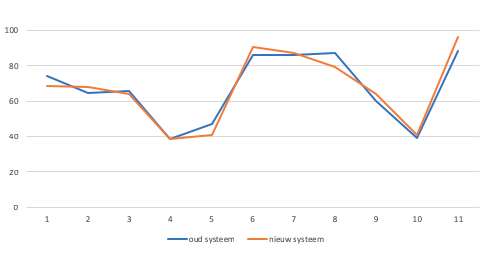
\includegraphics[height=9cm]{img/grafiek.png}
	\caption{Resultaat batch testen}
	\label{fig:batchtest}
\end{figure}



%paramaters

%basic utterances per intent

%Voor toepassing systeem

%2 zinnen niet herkent

% Voeg hier je eigen hoofdstukken toe die de ``corpus'' van je bachelorproef
% vormen. De structuur en titels hangen af van je eigen onderzoek. Je kan bv.
% elke fase in je onderzoek in een apart hoofdstuk bespreken.

%\input{...}
%\input{...}
%...

%%=============================================================================
%% Conclusie
%%=============================================================================

\chapter{Conclusie}
\label{ch:conclusie}

% TODO: Trek een duidelijke conclusie, in de vorm van een antwoord op de
% onderzoeksvra(a)g(en). Wat was jouw bijdrage aan het onderzoeksdomein en
% hoe biedt dit meerwaarde aan het vakgebied/doelgroep? 
% Reflecteer kritisch over het resultaat. In Engelse teksten wordt deze sectie
% ``Discussion'' genoemd. Had je deze uitkomst verwacht? Zijn er zaken die nog
% niet duidelijk zijn?
% Heeft het onderzoek geleid tot nieuwe vragen die uitnodigen tot verder 
%onderzoek?

Wat we uit dit onderzoek kunnen besluiten is dat er wel degelijk een manier is om te realiseren wat er wordt gevraagt in de onderzoeksvraag. Wel is dit op een andere manier dan dat verwacht was. Er was verwacht dat minstens één van de onderzochte frameworks een API zou hebben die toegankelijk genoeg zou zijn voor dit te realiseren. Wat bleek was dat dit niet het geval was, geen enkele van de frameworks had deze gewenste API-call of was er niet genoeg informatie in de respons van deze call voor dit allemaal te realiseren op deze manier.

Wat wel bleek uit dit onderzoek is dat er een andere manier was om dit te realiseren. Eén framework genaamd LUIS had andere API-calls met de benodigde informatie om de input van de gebruikers rechtsstreeks op te vangen en met de info die LUIS meegaf, zo de utterance te koppelen met de juiste intent. Enkel LUIS was in staat om dit op deze manier te doen omdat deze per utterances meer info gaf dan andere frameworks. Juist dit was noodzakelijk om te kunnen onderzoeken of LUIS zeker genoeg was dat een utterance bij een bepaalde intent past. Bij de andere frameworks kan deze controle niet worden gedaan omdat er niet genoeg info wordt weergegeven.

Uit de testen die zijn gedaan met de proof of concept is gebleken dat 50 percent van de inputs van de gebruiker niet meer in de 'Review endpoint utterances' kwam maar rechtstreeks werd gekoppeld aan de juiste intent. Hier is ook gecontroleerd geweest wat de invloed is op de accuraatheid van LUIS. De resultaten hiervan zijn positief uitgevallen. De accuraatheid is niet gedaald, deze is zelf lichtjes gestegen. Er was verwacht dat deze wat meer zou stijgen maar door de beperkte hoeveelheid utterances per intent is dit niet zo gestegen. Dit zal meer en meer beginnen stijgen vanaf er meer en meer verschillende utterances zullen komen per intent.

Wat er verwacht was van het onderzoek was een automatisatie van 10 tot 30 percent. Wat uit het onderzoek is gebleken, is dat automatisatie effectief mogelijk is met zelf een beter resutaat dat werd verwacht. Uit de opzet en de tests was maar liefst 50 percent automatisch toegewezen aan de intent. Er kunnen altijd nog aanpassingen gedaan worden aan de parameters voor de controle van de utterance voor dit eventueel nog beter te maken maar er moet altijd wat speling zijn voor eventuele fouten op te vangen zodat deze kunnen vermeden worden.

Wat er in een vervolgonderzoek nog kan gebeuren is het onderzoeken van intents met meer ingewikkeldere utterances, bijvoorbeeld utterances met meer dan 1 entity. Hier zou ook beter kunnen gecontroleerd worden of deze entities correct uit de utterance worden gehaald. Een intent met nog maar weinig utterances zal meer last kunnen hebben met deze er correct uit te halen dan intents met al een grote verscheidenheid aan utterances. Ook zouden er meerdere LUIS applicaties kunnen gestest worden, met elk een vershillend doen en verschillende testdata, eventueel een veel grotere testdataset. Ook bij deze controleren in welke mate de input van de gebruiker al automatisch gelinkt wordt met de correcte intent.





%%=============================================================================
%% Bijlagen
%%=============================================================================

\appendix
\renewcommand{\chaptername}{Appendix}

%%---------- Onderzoeksvoorstel -----------------------------------------------

\chapter{Onderzoeksvoorstel}

Het onderwerp van deze bachelorproef is gebaseerd op een onderzoeksvoorstel dat vooraf werd beoordeeld door de promotor. Dat voorstel is opgenomen in deze bijlage.

% Verwijzing naar het bestand met de inhoud van het onderzoeksvoorstel
\input{../voorstel/voorstel-inhoud}

%%---------- Andere bijlagen --------------------------------------------------
% TODO: Voeg hier eventuele andere bijlagen toe
\chapter{Testdata}
AddMore
\begin{itemize}
	\item Can you please add 5 more?
	\item I want to add 3 more.
	\item Will you please add 4 more?
	\item Let's add 2 more.
	\item Add 8 more.
	\item I need 3 more.
\end{itemize}

ClearBasket
\begin{itemize}
	\item I want to clear my basket.
	\item Can you remove my basket?
	\item I want my basket to be empty.
	\item Can you delete everything from my basket?
	\item Clear my basket.
	\item Empty my shopping list.
\end{itemize}

DeleteItem
\begin{itemize}
	\item Can you remove this from my shopping list?
	\item I want to remove this item.
	\item Please, delete this from my shopping list.
	\item Will you remove this from my basket?
	\item Delete item.
	\item Remove this.
\end{itemize}

FindItem
\begin{itemize}
	\item I want to add some salami.
	\item Can you find salami for me please?
	\item I would like to find 5 beers.
	\item I want to find some beers.
	\item I need 8 more beers please.
	\item I am looking for catfood.
\end{itemize}

Greeting
\begin{itemize}
	\item Hi, my name is Ivor.
	\item Good morning, I'm Ivor.
	\item Hello, how are you?
	\item Good evening.
	\item Hello, what's up?
	\item Hello.
\end{itemize}

Help
\begin{itemize}
	\item Please, I need help.
	\item Can you help me with this?
	\item What is this?
	\item I don't get it how this works.
	\item I want help.
	\item Please, help me.
\end{itemize}

RemoveMore
\begin{itemize}
	\item Can you remove these items?
	\item I want to remove this 2 times.
	\item Can you please remove this a couple of times?
	\item Remove 5 pieces from this item.
	\item Remove 8 items.
	\item Remove items.
\end{itemize}

ShowBasket
\begin{itemize}
	\item I want to see my basket.
	\item Can you show me my shopping list?
	\item What's in my cart?
	\item Please, show my cart.
	\item Show my shopping basket?
	\item Please, show me my basket.
\end{itemize}

ShowProfile
\begin{itemize}
	\item I want to see my profile.
	\item Can you show me my information?
	\item What's my profile information?
	\item Show my profile.
	\item What's my name.
	\item Show my username.
\end{itemize}

Stop
\begin{itemize}
	\item Can you stop?
	\item Please start over again.
	\item I want to exit.
	\item Let's quit.
	\item Can I stop?
	\item Make it stop.
\end{itemize}

UpdateProfile
\begin{itemize}
	\item I want to update my name.
	\item Can you change my username?
	\item Update my profile please.
	\item Will you change my username?
	\item Change my name.
	\item Update my username.
\end{itemize}

%%---------- Referentielijst --------------------------------------------------

\printbibliography[heading=bibintoc]

\end{document}
